\documentclass[11pt]{article}
\usepackage[margin=1in]{geometry}
\usepackage{amsmath,amssymb}
\usepackage{booktabs}
\usepackage{tabularx}
\usepackage{longtable}
\usepackage{array}
\usepackage{enumitem}
\usepackage{xcolor}
\usepackage{hyperref}
\usepackage{caption}
\usepackage{float}
\usepackage{graphicx}
\usepackage[most]{tcolorbox}
\usepackage{titlesec}
\usepackage{microtype}
\hypersetup{
  colorlinks=true,
  linkcolor=black,
  citecolor=black,
  urlcolor=black,
  pdftitle={Quantity and Quality: A Proposed Exergy-Factor Reporting Framework for Energy Systems},
  pdfauthor={Christopher DiMurro},
  pdfsubject={A proposed operational framework for reporting energy quantity with Exergy Factor},
  pdfkeywords={exergy, Exergy Factor, energy quality, energy reporting, thermodynamics}
}
\newif\ifpreprintquickreference
\ifdefined\journalversion
  \preprintquickreferencefalse
\else
  \preprintquickreferencetrue
\fi
\setlength{\parskip}{0.45em}
\setlength{\parindent}{0em}
\setlist[itemize]{leftmargin=1.2em,itemsep=0.15em,topsep=0.25em}
\setlist[enumerate]{leftmargin=1.4em,itemsep=0.2em,topsep=0.25em}
\setlength{\emergencystretch}{3em}
\sloppy

\newcommand{\fx}{f_X}
\newcommand{\XA}{X_A}
\newcommand{\XdotA}{\dot{X}_A}
\newcommand{\Xap}{X_{\mathrm{applied}}}
\newcommand{\Xdotap}{\dot{X}_{\mathrm{applied}}}
\newcommand{\Xdest}{\dot{X}_{\mathrm{dest}}}
\newcommand{\etaloss}{\eta_X}
\newcommand{\thetaloss}{\theta_{\mathrm{loss}}}
\newcommand{\omegaloss}{\omega_{\mathrm{loss}}}
\newcommand{\carrier}{\mathrm{carrier}}
\newcommand{\MWh}{\mathrm{MWh}}
\newcommand{\MW}{\mathrm{MW}}
\newcommand{\MWex}{\mathrm{MW\_ex}}
\newcommand{\MWhhex}{\mathrm{MWh\_ex}}
\newcommand{\degC}{^{\circ}\mathrm{C}}


\definecolor{QBlue}{HTML}{EAF3FA}
\definecolor{QBlueFrame}{HTML}{2F5F8F}
\definecolor{QGreen}{HTML}{EEF8F0}
\definecolor{QGreenFrame}{HTML}{3B7A57}
\definecolor{QAmber}{HTML}{FFF7E6}
\definecolor{QAmberFrame}{HTML}{A66A00}
\definecolor{QGray}{HTML}{F4F4F4}
\definecolor{QGrayFrame}{HTML}{555555}

\newtcolorbox{principlebox}[1]{colback=QBlue,colframe=QBlueFrame,arc=1.5mm,boxrule=0.7pt,left=6pt,right=6pt,top=5pt,bottom=5pt,title=\textbf{#1}}
\newtcolorbox{rulebox}[1]{colback=QAmber,colframe=QAmberFrame,arc=1.5mm,boxrule=0.7pt,left=6pt,right=6pt,top=5pt,bottom=5pt,title=\textbf{#1}}
\newtcolorbox{contribbox}[1]{colback=QGreen,colframe=QGreenFrame,arc=1.5mm,boxrule=0.7pt,left=7pt,right=7pt,top=6pt,bottom=6pt,title=\textbf{#1}}
\newtcolorbox{infobox}[1]{colback=QGray,colframe=QGrayFrame,arc=1.5mm,boxrule=0.6pt,left=7pt,right=7pt,top=6pt,bottom=6pt,title=\textbf{#1}}

\title{\textbf{Quantity and Quality:}\\[0.4em]\textbf{A Proposed Exergy-Factor Reporting Framework for Energy Systems}}
\author{Christopher DiMurro\\Independent Researcher, Exergy Lab\\\href{mailto:chrisdimurro@gmail.com}{chrisdimurro@gmail.com}}
\date{August 2026}

\begin{document}
\maketitle

\begin{abstract}
First-law scalar energy accounting, expressed in joules, kilowatt-hours, megawatt-hours, quads, barrels-of-oil-equivalent, and related quantities, does not encode the second-law distinction between energy magnitude and accessible work potential unless an additional quality field is provided. Classical exergy analysis restores that distinction, but routine adoption has been limited by reference-state dependence, carrier-specific terminology, data requirements, and the perceived burden of full thermodynamic accounting. The result is a persistent operational gap between thermodynamic rigor and the low-overhead reporting interfaces used by plant engineers, utility managers, regulators, market designers, and investors.

This paper proposes a dual-layer framework for closing that gap. The \textit{physics layer} preserves carrier-level thermodynamics. It defines the intensive carrier potential as the exergy voltage, $\Delta\Phi_A^{(C)} = dX_A/dC$, and uses it to recover the carrier-current relation $\dot{X}_A = \dot{C}\Delta\Phi_A^{(C)}$, which can be written at a reporting boundary as $\dot{X}_A=f_X\dot{E}$. The \textit{interface layer} compresses that physics into a practical reporting token, $(E_{\mathrm{carrier}}, f_X)$, where $E_{\mathrm{carrier}}$ is a first-law energy quantity with explicit carrier and basis context, such as \texttt{MWh\_e}, \texttt{MWh\_th}, or \texttt{MWh\_HHV\_CH4}, and $f_X$ is the Exergy Factor, the accessible work potential per unit reported energy at the declared boundary. The factor exposes the stream's thermodynamic distinguishability from its reference rather than introducing distinguishability as a second multiplier. An optional end-use account then separates primary, secondary, final, and useful energy from the corresponding physical exergy stages, Applied Exergy at the device-to-task boundary, and the non-energy service outcome.

Five Fidelity Tiers, F0 through F4, allow the notation to scale from conventional scalar reporting, through presumptive lookup factors, asset-specific metadata, dynamic interval computation, and full state-vector engineering analysis without changing the public interface. The paper also defines optional diagnostics: Exergy Capital Efficiency for capital screening, and the Exergy Loss Angle, $\theta_{\mathrm{loss}}=\operatorname{atan2}(X_{\mathrm{lost}},X_{\mathrm{useful,out}})$, as a bounded display coordinate derived from second-law efficiency. The angle is not a new thermodynamic property; it is a visualization of retained versus lost useful work potential over a declared boundary and interval.

The framework is demonstrated with public XAI4HEAT district-heating telemetry. Four processed substations, covering 51{,}592 synchronized 15-minute intervals from the 2024--2025 heating season, are converted into dynamic F3 Exergy Factor records using measured primary supply temperature, measured ambient temperature, and the reported thermal-delivery field as an interval weight. The delivery-weighted portfolio Exergy Factor is 0.216 with a dynamic ambient sink and 0.173 with a fixed $20\degC$ sink. A supply-return sensitivity check shows that an integrated primary water-stream model gives 0.172, while a secondary-side proxy gives 0.125, reinforcing that the public token must carry method and tier metadata. The empirical demonstration is limited to thermal district-heating telemetry and does not validate the chemical-carrier registry or optional diagnostic metrics. The central practical claim is therefore narrow and operational: every reported energy quantity should carry an Exergy Factor, and supply, demand, storage, and conversion pathways should be matched by both quantity and quality.
\end{abstract}

\ifpreprintquickreference
\newpage
\begin{tcolorbox}[colback=white,colframe=black,arc=1.2mm,boxrule=0.8pt,left=8pt,right=8pt,top=6pt,bottom=6pt]
\footnotesize
\setlength{\parskip}{0.1em}
\setlength{\abovedisplayskip}{0.25em}
\setlength{\belowdisplayskip}{0.25em}
{\centering\Large\bfseries Quick Reference\par}\vspace{0.4em}
\textbf{Keywords:} exergy; Exergy Factor; exergy voltage; Exergy Loss Angle; typed energy reporting; energy quality; energy grade; multi-carrier energy systems; proposed reporting protocol; thermodynamic diagnostics.\par\vspace{0.4em}

\textbf{Two-layer architecture.} The physics layer preserves thermodynamic rigor across carriers. The interface layer compresses the result into a scannable operational token.

\textbf{Primary reporting token.} Every energy quantity is reported as
\begin{equation*}
(E_{\carrier},\,\fx),
\end{equation*}
where $E_{\carrier}$ carries a carrier suffix and $\fx=\XA/E$ is accessible work potential per unit reported energy at a declared boundary. For rates, $P_{\carrier},\fx$ is used and $\fx=\XdotA/P$. The factor is not an efficiency; when the denominator is an accounting basis such as LHV, $\fx$ can exceed 1.

\textbf{Carrier Registry.} Underscore-delimited suffixes identify the carrier and, where required, the basis: \texttt{MWh\_e} for electricity, \texttt{MWh\_m} for mechanical or shaft work, \texttt{MWh\_th} for thermal energy, \texttt{MWh\_HHV\_CH4} for methane on higher heating value basis, \texttt{MWh\_LHV\_CH4} for methane on lower heating value basis, and \texttt{MWh\_HHV\_H2} for hydrogen on higher heating value basis.

\textbf{Universal flow law.}
\begin{equation*}
\XdotA = \dot{C}\Delta\Phi_A^{(C)} = \fx\dot{E},\qquad \Delta\Phi_A^{(C)}=\frac{d\XA}{dC}.
\end{equation*}
For multi-carrier systems, use the summed form $\XdotA = \sum_j \dot{C}_j\Delta\Phi_A^{(C_j)}$.

\textbf{Distinguishability.} Exergy measures a work-bearing distinction between a stream and its declared environment or task boundary. At equilibrium the states are indistinguishable, the gradient vanishes, and $\fx=0$. Distinguishability is therefore the physical basis of $\fx$, not a second multiplier.

\textbf{End-use chain.} Primary energy may become secondary energy in a transformed, transportable carrier before final delivery; useful energy then leaves the end-use device. The exergy crossing the last device-to-task boundary is called \emph{Applied Exergy}, $\Xap$, in this framework. It corresponds to useful exergy or useful work in societal exergy accounting, but is not the same quantity as useful energy. Statistical substitution equivalents must remain labelled and are not physical exergy streams.

\textbf{Thermal streams.} For a constant-temperature source $T_h$ and sink $T_c$, with entropy as carrier,
\begin{equation*}
\Delta\Phi_A^{(S)} = T_h-T_c,\qquad f_{X,Q} = 1-\frac{T_c}{T_h}.
\end{equation*}
Non-isothermal streams require integration or a higher Fidelity Tier.

\textbf{Default reference.} Unless otherwise declared, this paper uses $T_0=20\degC$ or 293.15 K and $p_0=101.325$ kPa for thermal examples. Other sinks are allowed, but must be declared.

\textbf{Five Fidelity Tiers.} F0 scalar legacy; F1 presumptive lookup; F2 asset-specific; F3 dynamic interval; F4 full vector audit. F0 through F4 are used to avoid conflict with $T_0$, the reference temperature.

\textbf{Illustrative Reference Exergy Factors, sink at $20\degC$ unless noted.}
\begin{center}
\begin{tabularx}{0.88\linewidth}{@{}lX@{}}
\toprule
Electricity & $\fx = 1.0$ \\
Mechanical or shaft work & $\fx = 1.0$ \\
Heat at $150\degC$ & $\fx = 0.307$ \\
Heat at $80\degC$ & $\fx = 0.170$ \\
Heat at $40\degC$ & $\fx = 0.064$ \\
Methane, HHV basis & $\fx^{\mathrm{HHV}} \approx 0.93$ \\
Hydrogen, HHV basis & $\fx^{\mathrm{HHV}} \approx 0.83$ \\
\bottomrule
\end{tabularx}
\end{center}

\textbf{Geometric diagnostic.} $\XA=E\fx$; $X_{\mathrm{lost}}=X_{\mathrm{in}}-X_{\mathrm{useful,out}}$; $\thetaloss=\operatorname{atan2}(X_{\mathrm{lost}},X_{\mathrm{useful,out}})$. The angle is a display coordinate derived from second-law efficiency, not a new thermodynamic state variable.

\textbf{Matching rule.} Supply $(E_s,f_{X,s})$ and demand $(E_d,f_{X,d})$ should be matched in both quantity and Exergy Factor.
\end{tcolorbox}
\newpage
\fi
\section{Introduction}

\subsection*{The scalar reporting gap}

Modern energy reporting treats joules as joules. International accounting systems, national statistical agencies, corporate sustainability disclosures, building energy codes, utility tariffs, engineering spreadsheets, and energy-transition dashboards converge on a first-law scalar quantity as the standard unit of analysis: kilowatt-hours, megawatt-hours, terawatt-hours, quads, barrels-of-oil-equivalent, tonnes of oil equivalent, or similar measures. This convention is simple, additive, and compatible with the first law of thermodynamics.

The convention is also incomplete for operational decision-making. One megawatt-hour of electricity, one megawatt-hour of natural gas reported on a higher heating value basis, one megawatt-hour of heat at $80\degC$, and one megawatt-hour of heat at $40\degC$ are not equivalent useful-work resources. They contain the same scalar energy magnitude, but they do not provide the same accessible work potential, service flexibility, or downstream option value. The second law has been understood for more than a century; what remains underdeveloped is a lightweight, standards-compatible reporting layer that makes work-potential grade visible at the same moment, and in nearly the same format, as energy quantity.

The same interface gap appears in power reporting. A plant may consume megawatts of electricity, a heat loop may deliver megawatts of thermal output, and a tariff may charge for peak kilowatts. These rate quantities describe how fast energy crosses a boundary. They do not describe how much useful work potential crosses that boundary. A megawatt of electricity, a megawatt of heat at $80\degC$, and a megawatt of heat at $40\degC$ can be equal as first-law rates while being sharply unequal as second-law resources.

\subsection*{The paradox of efficiency}

The problem is most visible in heating. A direct electric-resistance heater delivering low-temperature space heat is often reported as approximately 99 percent efficient on a first-law basis: nearly every joule of electrical input becomes a joule of thermal output. The second-law account is almost the inverse. High-grade electricity has an Exergy Factor near unity at the point of use. Low-temperature space heat may have an Exergy Factor near 0.06 when referenced to a $20\degC$ sink and a $40\degC$ delivered temperature. The device satisfies the energy quantity, but it destroys or degrades most of the accessible work potential consumed to produce that service. What the first law presents as nearly perfect, the second law identifies as severe mismatch.

This paradox is structural, not numerical. It appears whenever a high-work-potential stream is used for a low-work-potential service without a cascade, storage, or upgrading logic that preserves useful options elsewhere. District heating systems can report megawatt-hours of delivered heat while hiding whether those megawatt-hours were delivered at an unnecessarily high temperature. Industrial sites can list waste-heat resources in aggregate megawatt-hours while obscuring which streams have realistic recovery value. Hydrogen, methane, synthetic fuels, and storage assets can be compared on a nominal energy basis while silently mixing lower heating value, higher heating value, chemical exergy, and service-specific work potential. Scalar accounting does not encode these distinctions unless an additional quality field is provided.

\subsection*{The operational gap}

Classical exergy analysis has been capable of resolving these confusions for decades. Kotas, Szargut, Bejan, and related thermodynamic literature established the mathematical machinery for distinguishing energy from useful work potential \cite{kotas1985,szargut2005,bejan2016}. The problem is not that the second law lacks analytical tools. The problem is that the tools have not become a routine reporting interface. Three barriers recur. First, exergy is reference-dependent, and the selected environment, sink, boundary, and service materially affect the reported value \cite{gaudreau2012}. Second, conventional exergy treatments are often carrier-isolated, with separate terminology and calculation habits for thermal, chemical, mechanical, electrical, and pressure-driven streams. Third, full exergy balances require data and expertise that exceed the budget of many operational reporting workflows.

The unmet need is therefore not a more sophisticated exergy method. It is a practical reporting layer that is rigorous enough to be defensible, simple enough to be adopted, and structured enough to scale from a spreadsheet lookup to full engineering analysis without changing its public interface.

This paper proposes such a layer. The framework is organized as a two-layer architecture. The physics layer preserves the full thermodynamic backend: accessible exergy as a relational quantity, exergy voltage as the carrier-level intensive variable, a universal flow law, and a unified carrier matrix. The interface layer converts that backend into a typed reporting token, $(E_{\mathrm{carrier}},\fx)$, five Fidelity Tiers, a Carrier Registry, a declare-once basis block, and optional diagnostics for matching, visualization, and capital screening. The operational goal is not to replace existing meters, tariffs, ISO 50001 energy management systems, IPMVP measurement and verification reports, or ISO 14040 life-cycle inventories \cite{evo2022,iso14040,iso50001}. The goal is to attach a minimal second-law field to the first-law quantities already being reported.


\subsection*{Novel contributions}

This work builds on established exergy theory and on the exergy-voltage concept introduced by Li et al. \cite{li2022}, but contributes the following operational reporting elements:
\begin{enumerate}[leftmargin=1.4em]
\item A dual-layer architecture that preserves full carrier-level thermodynamics in a physics layer while exposing a compact interface token, $(E_{\mathrm{carrier}},\fx)$.
\item The Exergy Factor, $\fx=\XA/E$ or $\XdotA/\dot{E}$, as a declared-context scalar for cross-carrier comparison without erasing carrier identity.
\item Five Fidelity Tiers, F0 through F4, that allow the same token to scale from legacy scalar reporting to full vector audit.
\item A Carrier Registry with underscore-delimited typed suffixes and declare-once basis blocks for industrial data schemas.
\item A minimum machine-readable record, conformance fields, and registry-version convention for data systems.
\item Exergy Capital Efficiency, $\mathrm{ECE}=\Delta X_A/\mathrm{capital\ cost}$, as a thermodynamic screen for capital allocation.
\item The Exergy Loss Angle, $\thetaloss=\operatorname{atan2}(X_{\mathrm{lost}},X_{\mathrm{useful,out}})$, and Loss Angle Velocity, $\omegaloss$, as optional geometric diagnostics for dashboards and prognostics.
\item A Thermodynamic Honesty Rule and supply-demand matching rule that connect first-law metering to second-law interpretation.
\end{enumerate}
Li et al. provide the network-theoretic bridge. This paper generalizes the exergy-voltage idea into the carrier-level backend of a proposed reporting protocol and adds the interface, registry, fidelity, diagnostic, empirical-demonstration, and conformance machinery needed for routine adoption.

The remainder of the paper develops the framework in that order. Section 2 positions the work against classical exergy analysis and the multi-carrier network literature. Section 3 establishes the physics layer. Sections 4 and 5 define the interface layer and its Fidelity Tiers. Section 6 preserves the stream-versus-process separation and supply-demand matching machinery. Section 7 treats the Exergy Loss Angle as an optional diagnostic visualization of second-law efficiency. Section 8 gives illustrative applications and screening examples. Section 9 provides an empirical F3 proof-of-implementation using public XAI4HEAT district-heating data. Section 10 delimits the framework's epistemological boundaries and institutional adoption constraints. Section 11 concludes with the central claim: energy systems should report not only how much energy they move, store, or consume, but how much useful work potential remains accessible.

\section{Foundational Literature and the Network Bridge}

\subsection*{Classical exergy and its operational ceiling}

Energy is conserved. Exergy is not. In a process that generates entropy, total energy is conserved but accessible useful work potential is destroyed. For a reference environment at $T_0$, the Gouy-Stodola theorem gives
\begin{equation}
X_{\mathrm{dest}} = T_0 S_{\mathrm{gen}},
\end{equation}
and, in rate form,
\begin{equation}
\dot{X}_{\mathrm{dest}} = T_0 \dot{S}_{\mathrm{gen}} \ge 0.
\end{equation}
For a simple closed system relative to an environment $(T_0,p_0)$, physical exergy is commonly written as
\begin{equation}
X = (U-U_0)+p_0(V-V_0)-T_0(S-S_0),
\end{equation}
with chemical, kinetic, and potential contributions added as required. For steady-flow streams, specific flow exergy includes enthalpy, entropy, chemical-potential, kinetic, and potential terms.

These formulas are indispensable for engineering design. They are also too heavy to serve directly as the public language of every energy report, invoice, operating dashboard, planning model, or policy table. The exergy literature has long recognized that reference-environment selection affects interpretation and sustainability decisions \cite{gaudreau2012}. Energy quality and energy grade literature has similarly identified the need to generalize energy-quality concepts across energy forms while acknowledging terminology and benchmark ambiguity \cite{chen2022}. Chemical exergy tables provide essential values for fuels and elements, but they carry their own reference-environment conventions \cite{morris1986,rivero2006,szargut2005}. These are not defects in exergy. They are signs that exergy is a relational quantity.

Chen et al. \cite{chen2022} provide the closest prior conceptual neighbor by synthesizing energy quality and energy grade across forms of energy. Their work identifies the need for broader quality metrics, but it does not specify a compact operational reporting token, fidelity-scaled implementation tiers, a machine-readable carrier registry, or conformance metadata for industrial systems. In that sense, Chen et al. diagnose the problem class, while the present paper proposes a deployable reporting protocol for carrying those quality concepts into spreadsheets, SCADA tags, ISO 50001 performance indicators, and IPMVP-style measurement-and-verification reports.

The practical ceiling of classical exergy is therefore institutional as much as mathematical. A full exergy balance can answer a detailed engineering question, but most organizations need a smaller question answered repeatedly: when a stream is reported as a megawatt-hour, how much useful work potential does that quantity actually represent at the declared boundary? This paper treats that smaller question as the basis for a proposed operational reporting protocol.

\subsection*{The multi-carrier network bridge}

The key bridge between classical exergy and operational multi-carrier reporting is the exergy-voltage work of Li et al. \cite{li2022}. Their formulation analyzes exergy-flow distributions in regional integrated energy systems using voltage-like and impedance-like analogies adapted from electrical network theory. The importance of that contribution is not merely terminological. It shows that exergy can be represented as a network quantity governed by carrier-agnostic flow relationships across electricity, heat, and gas networks.

This paper builds directly on that bridge, but with a different objective. Li et al. establish the network-theoretic viability of unified exergy modeling. The present work translates that type of unified physical architecture into a reporting interface designed for plants, markets, public datasets, storage comparisons, district-energy systems, and standards bodies. In this sense, the paper is not claiming to discover the second law, nor to replace classical exergy analysis, nor to make exergy independent of reference conditions. It is proposing a standardized operational abstraction: the typed energy quantity plus Exergy Factor.

\subsection*{Positioning}

The proposed framework sits between two extremes. On one side is conventional first-law scalar reporting, which is easy to adopt but incomplete when energy grade matters. On the other side is full exergy analysis, which is rigorous but too burdensome for routine reporting. The proposed protocol is a translation layer between those poles. It preserves the physics through declared carriers, boundaries, reference sinks, bases, and fidelity tiers. It exposes the operational result through the compact token $(E_{\mathrm{carrier}},\fx)$.

The intended use is supplemental rather than substitutive. In an ISO 50001 energy management system, the Exergy Factor can become an additional energy performance indicator. In IPMVP-style measurement and verification, savings can be reported as both energy savings and exergy savings. In ISO 14040 life-cycle inventory work, energy and material flows can carry thermodynamic quality attributes without replacing emissions, resource, or impact categories. In dispatch and markets, the same energy interval can carry both MWh and MWh\_ex fields. The framework extends existing accounting rather than asking institutions to abandon it.

\begin{table}[H]
\centering
\small
\caption{Positioning relative to adjacent literature and reporting systems.}
\label{tab:prior_work_positioning}
\begin{tabularx}{\linewidth}{@{}p{0.28\linewidth}p{0.32\linewidth}X@{}}
\toprule
Prior work or system & What it provides & What this paper adds \\
\midrule
Classical exergy analysis \cite{kotas1985,szargut2005,bejan2016} & Rigorous thermodynamic accounting, reference-environment methods, and process-level exergy balances. & A lightweight reporting interface that can be attached to existing first-law quantities without requiring every report to become a full exergy audit. \\
Energy quality and energy grade literature \cite{chen2022} & Conceptual quality metrics and recognition that energy forms differ in ability to perform useful work. & A typed token, Carrier Registry, Fidelity Tiers, and conformance metadata for operational datasets. \\
Exergy-voltage and integrated energy-system modeling \cite{li2022} & Network-theoretic exergy-flow modeling across electricity, heat, and gas systems. & A standards-compatible reporting layer for SCADA tags, tables, APIs, audits, and public datasets. \\
ISO 50001, IPMVP, and life-cycle reporting interfaces \cite{evo2022,iso14040,iso50001} & Energy management, savings verification, and structured environmental reporting. & A supplemental second-law quality field attached to the quantities those systems already collect. \\
\bottomrule
\end{tabularx}
\end{table}

\section{Unified Carrier Theory: The Physics Layer}

This section establishes the physical architecture that justifies the operational reporting protocol introduced later. The architecture rests on three elements: accessible exergy as a relational quantity bounded by a declared reporting context; a carrier-level intensive variable, the exergy voltage; and a universal carrier-current-times-potential structure that can be expressed for electricity, thermal streams, chemical carriers, pressure-driven flow, and mechanical work.

\subsection{Thermodynamic exergy, accessible exergy, and the Exergy Factor}

This paper distinguishes conventional thermodynamic exergy, $X$, from accessible or admissible exergy, $\XA$. Conventional exergy is the maximum useful work potential of a system relative to a declared reference environment under the assumptions of the thermodynamic model. Accessible exergy is the portion of that potential admitted by a declared reporting boundary, service requirement, carrier definition, and operationally available conversion path. A compact way to express the distinction is
\begin{equation}
\XA=\alpha_{\mathrm{access}}X,
\end{equation}
where $\alpha_{\mathrm{access}}$ is a declared boundary and pathway factor. In many operational cases $0\le \alpha_{\mathrm{access}}\le 1$, but it is not a universal material property; it is part of the reporting context. This distinction prevents the interface layer from quietly redefining classical exergy. The physics layer retains $X$ as the conventional thermodynamic quantity and uses $\XA$ when the report intentionally limits analysis to accessible or admissible pathways.

\textbf{Definition 1: Accessible exergy.} Accessible exergy, $\XA$, is the useful work potential of a stream at a specified reporting boundary, evaluated relative to the declared reference sink, service requirement, carrier definition, and operational constraints of the system being analyzed.

The word accessible is retained because operational reports often need to exclude pathways that are physically possible in principle but unavailable within the declared boundary. A waste-heat stream can have nonzero thermodynamic exergy but no recoverable site value if the site lacks a heat exchanger, sink, network, storage asset, or demand capable of using it. A fuel can have a stable tabulated chemical exergy but still be poorly matched to a particular service. The declared boundary and allowed conversion path are therefore part of the reported $\XA$ value, not hidden assumptions.

\textbf{Definition 2: Exergy Factor.} The Exergy Factor of an energy quantity is the accessible exergy per unit reported energy:
\begin{equation}
\fx = \frac{\XA}{E}.
\end{equation}
For a power flow, the same factor is accessible exergy rate per unit reported power:
\begin{equation}
\fx = \frac{\XdotA}{P}=\frac{\XdotA}{\dot{E}}.
\end{equation}
The factor can be written in units such as J\_ex/J, MW\_ex/MW, or MWh\_ex/MWh, but it is most often used as a dimensionless ratio once the reported basis is declared.

The Exergy Factor is not a second-law efficiency and is not guaranteed to lie between 0 and 1 under every accounting denominator. For thermal factors on a heat basis, $0\le \fx\le 1$ under ordinary positive-temperature assumptions. For chemical fuels reported on lower heating value or another partial accounting basis, $\fx$ may exceed 1 because the denominator is not the full thermodynamic work-potential inventory. A value above 1 is therefore a basis signal, not a violation of the second law.

\paragraph{Principle 1: Relational work potential.} Exergy is fundamentally relational, not absolute. It measures accessible difference: useful work potential exists only when a system has an accessible gradient relative to a sink, service, boundary condition, or allowed conversion path.

This relational property can also be stated as thermodynamic \emph{distinguishability}: exergy measures how far the target state remains distinguishable from the declared environment in temperature, pressure, composition, electrical or mechanical potential, radiation field, or another work-bearing coordinate \cite{ayres2006}. When the relevant state is identical to the environment, the distinction vanishes and so does its exergy. Distinguishability is not introduced here as an additional empirical coefficient. Doing so would count the same physical difference twice; the Exergy Factor already quantifies it on the reported energy basis.

\subsection{Primary, secondary, final, useful, and Applied Exergy accounting}

Standard energy accounting distinguishes primary energy at the resource or statistical supply boundary, secondary energy after conversion into a transportable carrier, final energy delivered to an end user, and useful energy leaving an end-use conversion device \cite{ieaglossary,owiddefinitions,brockway2024}. Electricity at generator output, refined petroleum products leaving a refinery, and heat entering a district network are secondary-energy examples. The secondary boundary is optional in a compact account because some datasets do not publish it separately and some carriers pass from production to final delivery without a useful intervening aggregate.

Each physical boundary can also carry exergy. This paper uses \emph{Applied Exergy} for the exergy that reaches and crosses the last device-to-task boundary:
\begin{equation}
E_{\mathrm{primary}}\longrightarrow E_{\mathrm{secondary}}\longrightarrow E_{\mathrm{final}}\longrightarrow E_{\mathrm{useful}}\longrightarrow \mathcal{S},
\end{equation}
\begin{equation}
X_{\mathrm{primary}}\longrightarrow X_{\mathrm{secondary}}\longrightarrow X_{\mathrm{final}}\longrightarrow \Xap,
\end{equation}
where $\mathcal{S}$ is the resulting energy service. In established societal exergy literature, $\Xap$ is commonly called useful exergy or useful work. The name Applied Exergy is used here to make the application boundary explicit and to prevent confusion with useful energy.

Useful energy and Applied Exergy are not interchangeable. Useful energy is the first-law output delivered by an end-use device and can contain both exergy and anergy. At a correctly specified useful-output boundary,
\begin{equation}
\Xap=E_{\mathrm{useful}}f_{X,\mathrm{useful}}
=X_{\mathrm{final}}\eta_{X,\mathrm{final\rightarrow applied}}.
\end{equation}
For shaft or electrical work, $f_{X,\mathrm{useful}}=1$ at the work-transfer boundary. For heat entering a liquid, gas, or occupied space, only the temperature-dependent exergy of the delivered heat is Applied Exergy; the remainder of the useful heat quantity is anergy. A heat pump can therefore deliver $E_{\mathrm{useful}}>E_{\mathrm{final}}$ while still satisfying $\Xap\le X_{\mathrm{final}}$ for a single-input exergy account.

The energy service is one step farther downstream and must remain separate from all energy and exergy columns. It is the societal outcome---for example cold beverages, occupied-space comfort hours, passenger-miles, tonne-metres, illumination, or completed material processing. Services are measured in outcome-specific units, cannot generally be aggregated in joules, and may also depend on buildings, vehicles, insulation, controls, time, and other non-energy inputs \cite{ieaglossary}. Applied-exergy intensity, $\Xap/\mathcal{S}$, and its inverse service productivity, $\mathcal{S}/\Xap$, may be reported only when the service unit and boundary are declared.

\paragraph{Statistical primary-energy conventions.} The label ``primary energy'' does not by itself establish a physical thermodynamic basis. Under the substitution method, non-fossil electricity is divided by an assumed thermal efficiency, $\eta_{\mathrm{reference}}$, to form a counterfactual fossil-input equivalent:
\begin{equation}
E_{\mathrm{primary,substitution}}=\frac{E_{\mathrm{electricity}}}{\eta_{\mathrm{reference}}}.
\end{equation}
For example, 100~TWh of electricity divided by 0.4 is reported as 250~TWh of substituted primary energy. This quantity can support historical statistical comparison, but no physical 250~TWh stream exists at the reported boundary. It must therefore be retained with an explicit accounting-method label and must not be inserted into $X=Ef_X$. Doing so would manufacture exergy from a counterfactual denominator.

The physical-energy-content method instead reports total energy supply without applying a fossil-equivalent adjustment to wind, solar photovoltaic, or hydropower electricity; thermal-input conventions remain for nuclear and heat-input technologies. The Energy Institute and Our World in Data moved their headline series from substitution to physical energy content or total energy supply in 2025--2026 \cite{owidprimary2026}. This is an accounting change, not a change to thermodynamics. A robust data interface should accept both conventions, preserve the source variable and method, and calculate exergy only for a disaggregated physical carrier with a defensible $f_X$. If a dataset reports only an aggregate energy mix without sufficient carrier composition, energy may be retained while exergy remains unreported.

\subsection{The exergy voltage}

\textbf{Definition 3: Exergy voltage.} Building on the exergy-voltage concept introduced by Li et al. \cite{li2022}, the carrier-level intensive variable of this framework is the exergy voltage. For a carrier $C$,
\begin{equation}
\Delta\Phi_A^{(C)}=\frac{d\XA}{dC}.
\end{equation}
The unit is J\_ex per unit carrier. The carrier may be electric charge, entropy, mole amount, volume, mass, or another physically measured extensive carrier. The exergy voltage is the accessible-potential difference associated with a differential increment of that carrier.

The carrier-normalized flow relation follows directly from the chain rule. If accessible exergy is transported by a carrier $C$ with carrier current $\dot{C}$, then
\begin{equation}
\XdotA = \frac{d\XA}{dt}=\frac{d\XA}{dC}\frac{dC}{dt}=\Delta\Phi_A^{(C)}\dot{C}.
\end{equation}

The derivation is simple, but its value lies in abstracting across carriers without erasing carrier identity. Electrical voltage is one member of a broader family of exergy-potential differences. Temperature difference becomes the exergy voltage when entropy is the carrier. Chemical potential difference becomes the exergy voltage when mole amount is the carrier. Pressure difference becomes the exergy voltage when volume is the carrier. Specific work potential becomes the exergy voltage when mass is the carrier.

\subsection{The universal flow law}

Combining the carrier-normalized form with the Exergy Factor definition yields the central equation of the framework:
\begin{equation}
\XdotA = \dot{C}\Delta\Phi_A^{(C)} = \fx\dot{E}.
\end{equation}
This is the single-carrier universal exergy-flow law. In the carrier formulation it is a definitional identity: carrier current multiplied by accessible carrier potential gives accessible exergy flow, and normalization by the reported energy rate gives $\fx$. When used as an operational model, however, it depends on the declared boundary, carrier aggregation, reference environment, and equilibrium assumptions. Coupled transport, finite heat exchange, composition changes, non-equilibrium states, and interacting carriers require the summed or full-vector forms below and may require F4 treatment.

The relation is the generalized analogue of electrical power,
\begin{equation}
\dot{W}=I\Delta V,
\end{equation}
where carrier current times carrier potential equals accessible exergy flow.

For multi-carrier systems, the correct generalization is a sum or vector inner product:
\begin{equation}
\XdotA = \sum_j \dot{C}_j\Delta\Phi_A^{(C_j)}.
\end{equation}
The scalar reporting token does not deny this vector structure. It projects the multi-dimensional carrier physics into a declared boundary-specific factor, $\fx$, for the purpose of operational reporting. The details remain available through metadata and Fidelity Tiers.

\subsection{The unified carrier matrix}

Table \ref{tab:carrier_matrix} maps the principal carriers to their exergy voltages and exergy-flow forms. The table does not imply that all carriers are physically identical. It shows that a common structural relationship, carrier current times accessible potential difference, governs the exergy flow in each case. For the entropy row, the unit K follows from the dimensional relation J\_ex/(J/K). For the mass-flow row, $\Delta\psi$ denotes a difference in specific flow exergy. For a nonreacting stream, a representative form is $\psi=(h-h_0)-T_0(s-s_0)+v^2/2+gz$, with chemical-potential terms added when composition is part of the state description.

\begin{table}[H]
\centering
\small
\caption{Unified carrier matrix: exergy voltage and exergy-flow forms across carriers.}
\label{tab:carrier_matrix}
\begin{tabularx}{\linewidth}{@{}p{0.18\linewidth}p{0.17\linewidth}p{0.24\linewidth}p{0.16\linewidth}X@{}}
\toprule
Carrier $C$ & Carrier current $\dot{C}$ & Exergy voltage $\Delta\Phi_A^{(C)}$ & Unit & Exergy flow \\
\midrule
Electric charge & $I=\dot{q}$ & Electric potential difference $\Delta V$ & J/C = V & $\XdotA=I\Delta V$ \\
Entropy & $\dot{S}$ & Temperature difference $T_h-T_c$ & K & $\XdotA=\dot{S}(T_h-T_c)$ \\
Mole amount & $\dot{n}_i$ & Chemical potential difference $\Delta\mu_i$ & J/mol & $\XdotA=\sum_i \dot{n}_i\Delta\mu_i$ \\
Volume & $\dot{V}$ & Pressure difference $\Delta p$ & J/m$^3$ = Pa & $\XdotA=\dot{V}\Delta p$ \\
Mass & $\dot{m}$ & Specific work potential $\Delta\psi$ & J/kg & $\XdotA=\dot{m}\Delta\psi$ \\
\bottomrule
\end{tabularx}
\end{table}

General photon exergy and information-theoretic work limits, including Landauer-type questions, are outside the routine plant-level Carrier Registry proposed here. Solar radiation is common enough in energy-system reporting to receive a limited registry token, but its $\fx$ value must be tied to a declared spectral, source-temperature, or receiver-boundary model rather than treated as a universal constant.

The reporting layer converts these carrier-specific potentials into a normalized factor, $\fx=\XA/E$ or $\fx=\XdotA/P$. The carrier suffix preserves identity; the Exergy Factor expresses boundary-specific work potential in a comparable form.

\subsection{Thermal streams as a worked example}

Thermal streams are the most common operational case where $\fx$ differs sharply from unity. Heat is energy transferred because of a temperature difference, but entropy is the natural extensive carrier for thermal exergy. For reversible heat transfer at temperature $T$,
\begin{equation}
\delta Q_{\mathrm{rev}} = T\,dS.
\end{equation}
For a constant-temperature heat source at $T_h$ delivering to a sink at $T_c$, the maximum reversible work rate is
\begin{equation}
\XdotA = \dot{Q}\left(1-\frac{T_c}{T_h}\right).
\end{equation}
Using $\dot{Q}=T_h\dot{S}$ gives
\begin{equation}
\XdotA=\dot{S}(T_h-T_c).
\end{equation}
The Exergy Factor of heat referenced to sink $T_c$ is therefore the Carnot factor:
\begin{equation}
f_{X,Q}=1-\frac{T_c}{T_h}.
\end{equation}

\paragraph{Principle 2: Thermal exergy voltage.} When entropy is the carrier, temperature difference is the thermal exergy voltage: $\Delta\Phi_A^{(S)}=T_h-T_c$.

With $T_c=20\degC=293.15$ K, heat at $T_h=80\degC=353.15$ K has
\begin{equation}
f_{X,Q}=1-\frac{293.15}{353.15}=0.170.
\end{equation}
Heat at $40\degC$ has $f_{X,Q}=0.064$, and heat at $150\degC$ has $f_{X,Q}=0.307$. These values are used as illustrative anchors throughout the paper. The default $T_0=20\degC$ is chosen here because it aligns with common building-service, HVAC, and district-heating boundary interpretations. Thermochemical tables often use $25\degC$, and oil-and-gas conventions sometimes use $15\degC$; those references are valid when declared. Figure \ref{fig:reference_temp_sensitivity} shows that the thermal factor for $80\degC$ heat shifts from 0.184 at a $15\degC$ sink to 0.156 at a $25\degC$ sink, which is small enough for screening but material enough for audited reporting.

\begin{figure}[H]
\centering
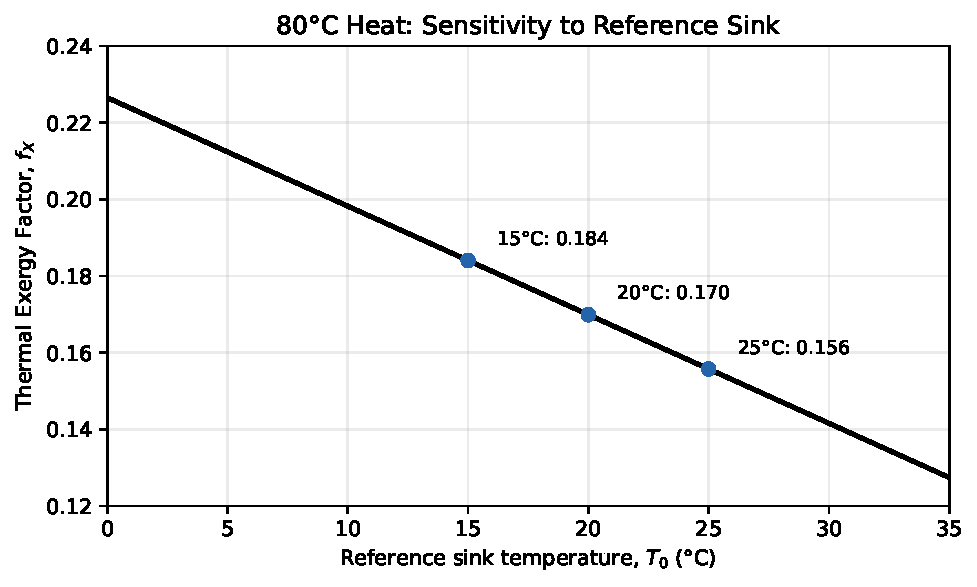
\includegraphics[width=0.78\linewidth]{reference_temp_sensitivity.pdf}
\caption{Sensitivity of the thermal Exergy Factor for $80\degC$ heat to the selected reference sink.}
\label{fig:reference_temp_sensitivity}
\end{figure}

This constant-temperature form is a reporting simplification, not a universal thermal exergy formula. Non-isothermal streams, finite heat exchangers, and distributed temperature profiles require integration over the temperature path. In the Fidelity Tier language introduced later, a fixed-temperature Carnot factor is suitable for F1 or F2 reporting when its assumptions are declared. F4 analysis uses the full temperature history and state description.

\subsection{Chemical carriers and energy-basis convention}

For chemical streams, the carrier is mole amount and the exergy voltage is chemical-potential difference. The exergy flow in a stream of species $i$ relative to a reference environment is
\begin{equation}
\XdotA = \sum_i \dot{n}_i\Delta\mu_i.
\end{equation}
For a tabulated standard chemical exergy on a mass basis,
\begin{equation}
\XdotA = \dot{m}e_{\mathrm{ch}},
\end{equation}
where $e_{\mathrm{ch}}$ is the specific chemical exergy. The Exergy Factor on a declared energy basis $h_B$ is
\begin{equation}
\fx^{(B)}=\frac{e_{\mathrm{ch}}}{h_B}.
\end{equation}
For the recommended higher-heating-value fuel token, this becomes
\begin{equation}
\fx^{\mathrm{HHV}}=\frac{e_{\mathrm{ch}}}{\mathrm{HHV}},
\end{equation}
which is the basis used for tokens such as \texttt{MWh\_HHV\_CH4} and \texttt{MWh\_HHV\_H2}. Common choices for $h_B$ are lower heating value, higher heating value, Gibbs free energy of reaction, and full chemical exergy. The denominator matters. For methane, lower heating value can yield $\fx^{\mathrm{LHV}}>1$ because the denominator is a selected accounting basis rather than the total accessible work inventory. This is not a physics violation. It is a basis effect.

Practical chemical implementation also requires more than choosing HHV or LHV. Reports should declare the reference-species model, the standard-state convention, and whether water is treated as liquid or vapor in hydrogen-related calculations. Szargut-style and Ahrendts/Rivero-style conventions can differ, and ambient composition, humidity, temperature, and pressure can affect chemical exergy values for atmospheric gases and gaseous fuels \cite{ertesvag2007}. The Carrier Registry and bracket metadata are the enforcement mechanism: a chemical token is incomplete if its basis and reference table are not recoverable.

For public-facing and cross-sector reporting, this framework recommends HHV as the default fuel basis because it is common in national energy statistics and keeps $\fx$ below unity for common combustion fuels. LHV remains valid where entrenched, but it must be visible in the carrier suffix, such as \texttt{MWh\_LHV\_CH4}. A report that writes only \texttt{MWh\_CH4} is incomplete.

For hydrogen on an HHV basis, $\fx^{\mathrm{HHV}}\approx 0.83$ is an engineering reference value using standard HHV and tabulated chemical exergy; exact values depend on the selected chemical-exergy table and water reference state \cite{rivero2006,morris1986}.

\subsection{The matching principle}

The physics layer has one direct operational implication: supply and demand should be matched by both energy quantity and Exergy Factor. A supply with the right MWh but the wrong $\fx$ can be operationally wasteful or technically insufficient.

\paragraph{Principle 3: Quantity-factor matching.} Energy systems should match supply and demand in both quantity and Exergy Factor. A megawatt-hour of supply and a megawatt-hour of demand are not equivalent unless their Exergy Factors are also compatible.

Principles 1 through 3 define the conceptual scope of the framework. Exergy is relational, thermal voltage is temperature difference when entropy is carrier, and supply-demand matching must address both energy magnitude and work-potential grade.

\section{The Core Reporting Protocol: The Interface Layer}

\subsection{The reporting tuple}

The interface layer compresses the physics layer into the primary operational token:
\begin{equation}
(E_{\carrier},\fx).
\end{equation}
The first term, $E_{\carrier}$, is the conventional first-law energy quantity with an explicit carrier and basis suffix. The second term, $\fx$, is the Exergy Factor associated with that quantity at the declared boundary. For power rates, the same structure is written as
\begin{equation}
(P_{\carrier},\fx).
\end{equation}
In plain operational syntax, examples include:
\begin{center}
\begin{tabular}{@{}ll@{}}
\texttt{100 MWh\_e, fx = 1.0} & delivered electricity, \\
\texttt{100 MWh\_th, fx = 0.170} & thermal energy at $80\degC$ relative to $20\degC$, \\
\texttt{100 MWh\_HHV\_CH4, fx = 0.93} & methane on HHV basis, \\
\texttt{100 MWh\_HHV\_H2, fx = 0.83} & hydrogen on HHV basis. \\
\end{tabular}
\end{center}
The notation is intentionally plain. It can fit in a spreadsheet cell, meter display, historian tag, CSV column, API payload, invoice, procurement table, or engineering report. The token is not meant to expose every physical assumption. It is meant to prevent scalar energy quantities from traveling alone.

\subsection{The Thermodynamic Honesty Rule}

The simplicity of the tuple creates a risk: a user may mistake $\fx$ for an intrinsic property of a stream or substance. That interpretation must be rejected. The Exergy Factor is not a material constant. It is a scalar projection of a relational thermodynamic state, computed under declared assumptions.

\paragraph{Thermodynamic Honesty Rule.} An Exergy Factor is valid only with respect to its declared carrier, reference sink, reporting boundary, energy basis, and allowed conversion path. The public interface may remain compact, but the audit layer must retain enough information to reproduce the factor at the claimed Fidelity Tier.

The Thermodynamic Honesty Rule is the bridge between usability and rigor. It allows the front-end notation to remain compact while preventing hidden assumptions from becoming invisible. A value such as \texttt{fx = 0.170} is not free-floating. It is meaningful because the carrier is thermal, the source temperature is $80\degC$, the reference sink is $20\degC$, and the calculation uses the constant-temperature Carnot factor.

\subsection{Typed units and the Carrier Registry}

The typed energy suffix is the immutable part of the reporting token. The proposed Carrier Registry uses underscore-delimited suffixes because they are readable by humans and safe for common databases, file names, industrial tags, historian variables, and message payloads.

\begin{table}[H]
\centering
\small
\caption{Core Carrier Registry entries and notation examples.}
\label{tab:carrier_registry}
\begin{tabularx}{\linewidth}{@{}p{0.27\linewidth}p{0.25\linewidth}X@{}}
\toprule
Suffix & Meaning & Reporting implication \\
\midrule
\texttt{MWh\_e} & Electricity & Treated as high-grade work potential at point of use; $\fx\approx 1$ unless boundary losses are included. \\
\texttt{MWh\_m} & Mechanical or shaft work & Separate from electricity to avoid using \texttt{\_e} for non-electrical work. \\
\texttt{MWh\_th} & Thermal energy & Temperature grade is represented by $\fx$ and, at F2 or above, bracket metadata rather than by separate low/high-temperature suffixes. \\
\texttt{MWh\_solar} & Solar radiation & Boundary is the receiving surface or aperture. $\fx$ requires a declared spectrum, source-temperature approximation, or radiation-exergy model; PV output is reported separately as \texttt{MWh\_e}. \\
\texttt{MWh\_HHV\_CH4} & Methane, HHV basis & Recommended default public fuel basis. \\
\texttt{MWh\_LHV\_CH4} & Methane, LHV basis & Explicitly labels a denominator that can yield $\fx>1$. \\
\texttt{MWh\_HHV\_NG} & Natural gas mixture, HHV basis & Use when the stream is a commodity gas mixture rather than pure methane; composition or tariff gas quality should be metadata at F2 or above. \\
\texttt{MWh\_HHV\_H2} & Hydrogen, HHV basis & Recommended public hydrogen basis for cross-sector comparisons. \\
\texttt{MWh\_HHV\_NH3} & Ammonia, HHV basis & Chemical-carrier token; toxicity, cracking pathway, and end-use boundary remain outside the suffix and must be metadata when relevant. \\
\texttt{MWh\_HHV\_CH3OH} & Methanol, HHV basis & Example liquid synthetic-fuel token; fuel purity and water content should be declared when material. \\
\texttt{MWh\_HHV\_diesel} & Diesel, HHV basis & Commodity petroleum-product token; grade, sulfur specification, bio-blend, and table source should be declared when material. \\
\texttt{MWh\_HHV\_gasoline} & Gasoline, HHV basis & Commodity petroleum-product token; blendstock, ethanol content, and table source should be declared when material. \\
\texttt{MWh\_HHV\_crude} & Crude oil, HHV basis & Heterogeneous feedstock token; API gravity, assay, sulfur content, and reference table should be metadata. \\
\texttt{MWh\_HHV\_coal} & Coal, HHV basis & Heterogeneous solid-fuel token; rank, moisture, ash, sulfur, and ultimate/proximate analysis should be metadata. \\
\texttt{MWh\_HHV\_biomass} & Biomass, HHV basis & Heterogeneous biogenic-fuel token; moisture content and feedstock class are mandatory for meaningful comparison. \\
\texttt{MWh\_fission} & Nuclear fission energy potential & Fuel-inventory token only. Reactor heat is reported as \texttt{MWh\_th}, and electricity as \texttt{MWh\_e}; isotope, enrichment, burnup, and fuel-cycle boundary must be declared. \\
\bottomrule
\end{tabularx}
\end{table}

The registry should be extendable, but new suffixes should be added only when they reduce ambiguity rather than encode details better handled as metadata. Single-suffix forms are preferred when the carrier is already clear: \texttt{MWh\_solar} denotes incident solar radiation at a declared receiving boundary, while solar photovoltaic output is \texttt{MWh\_e} and solar-thermal delivery is \texttt{MWh\_th}; \texttt{MWh\_fission} denotes nuclear fuel energy potential, while reactor heat is \texttt{MWh\_th} and nuclear electricity is \texttt{MWh\_e}. Steam, chilled water, and hot water usually remain \texttt{MWh\_th} with temperature, pressure, and phase metadata. Compressed air, cryogenic storage, pressure products, and specialized radiation models can receive suffixes when the reporting community defines stable boundaries and calculation rules. The proposed registry does not require the same suffix list forever. It requires that suffixes be declared, stable, parseable, and unambiguous.

\subsection{Bracket metadata}

The typed suffix does not eliminate metadata. It moves metadata into the appropriate tier. At F1, a lookup value may omit brackets because the value is presumed from a standard registry. At F2 and F3, bracket metadata provide auditability:
\begin{center}
\texttt{100 MWh\_th, fx = 0.170 [Th = 80C, T0 = 20C]}.
\end{center}
The bracket notation records the inputs needed to reproduce the value. For chemical fuels, the bracket may record the basis, table version, or reference condition:
\begin{center}
\texttt{100 MWh\_HHV\_CH4, fx = 0.93 [basis = HHV, table = standard]}.
\end{center}
For dynamic operation, the bracket may point to a time-series rule or dataset:
\begin{center}
\texttt{P\_th(t), fx(t) [Th = sensor.A, T0 = return.loop, interval = 15min]}.
\end{center}
The typed unit is the primary token. The brackets are tier-dependent verification metadata.

\subsection{Declare-once basis block}

To avoid clutter in large datasets, the framework supports a declare-once basis block. A report, table, API endpoint, or SCADA namespace can state shared assumptions once and then emit compact row-level tokens.

\begin{quote}\small\ttfamily
Reference sink: T0 = 20C, p0 = 101.325 kPa\\
Chemical basis: HHV unless suffix declares LHV\\
Thermal model: Carnot factor for constant-temperature streams\\
Carrier registry: underscore-delimited suffixes\\
Carrier registry version: 0.1\\
Fidelity tier: F2 unless otherwise marked\\[0.4em]
Rows can then be written compactly:\\
stream\_id, energy\_token, fx, metadata\\
HX-17, 240 MWh\_th, 0.307, Th = 150C\\
LOOP-04, 180 MWh\_th, 0.064, Th = 40C\\
NG-01, 500 MWh\_HHV\_CH4, 0.93, basis = HHV
\end{quote}

The declare-once block is essential for adoption because real industrial systems contain thousands of tags. The framework should not force every tag to repeat the same sink, pressure, table, and basis assumptions. It should require those assumptions to be declared at the correct scope.

\subsection{Minimum machine-readable record}

For standards use, the tuple should be carried by a small structured record rather than by prose alone. Table \ref{tab:min_record} gives the minimum fields proposed for a conforming machine-readable record. F0 records may leave \texttt{fx} null, but F1 through F4 records should populate the quality field and the metadata needed to interpret it.

\begin{table}[H]
\centering
\small
\caption{Minimum machine-readable fields for Exergy Factor reporting.}
\label{tab:min_record}
\begin{tabularx}{\linewidth}{@{}p{0.32\linewidth}p{0.14\linewidth}X@{}}
\toprule
Field & Required & Purpose \\
\midrule
\texttt{stream\_id} & Yes & Stable stream, meter, asset, or interval identifier. \\
\texttt{quantity} & Yes & First-law energy or rate value. \\
\texttt{unit} & Yes & Carrier-aware unit, such as \texttt{MWh\_th}, \texttt{MW\_e}, or \texttt{MWh\_HHV\_CH4}. \\
\texttt{fx} & F1+ & Exergy Factor at the declared boundary; null for F0. \\
\texttt{tier} & Yes & Fidelity Tier F0 through F4. \\
\texttt{reference} & F2+ & Reference sink, pressure, chemical basis, or reference environment. \\
\texttt{boundary} & F2+ & Physical or accounting boundary for the reported value. \\
\texttt{basis} & As applicable & Energy denominator and table convention, such as HHV, LHV, or thermal delivery. \\
\texttt{method\_id} & F2+ & Calculation method or model identifier used to compute $\fx$. \\
\texttt{timestamp} & F3+ & Interval timestamp or validity window. \\
\texttt{uncertainty} & As applicable & Reported uncertainty, confidence band, or propagation method. \\
\texttt{data\_quality\_flag} & F3+ & Missing-data, outlier, sensor-quality, or synchronization flag. \\
\texttt{carrier\_registry\_version} & Yes & Registry version used to parse the carrier suffix; this draft uses \texttt{0.1}. \\
\bottomrule
\end{tabularx}
\end{table}

\subsection{Reference-state handling}

The framework does not eliminate reference dependence. It standardizes how reference dependence is reported. A complete stream declaration can be written as
\begin{equation}
S=(E_{\carrier},\fx\mid R,B,O),
\end{equation}
where $R$ is the reference sink or environment, $B$ is the reporting boundary, and $O$ is the class of operationally available conversion paths. For operational front ends, the public token remains $(E_{\carrier},\fx)$. The metadata preserve reproducibility.

Two reference conventions should coexist. Comparable reporting, such as inventories, standards, benchmarking, and life-cycle analysis, should use a declared standard reference. Operational dispatch should use the local accessible sink or service boundary because that is what determines actual work potential. A district-heating operator may therefore publish both a standard $\fx$ for comparability and a dynamic $\fx(t)$ for control.

\section{Implementation Flexibility: The Five Fidelity Tiers}

A practical reporting protocol must support organizations with different data maturity. It must work for a policy table that has only energy totals, a plant operator with local temperatures, a district-energy network with continuous sensors, and an engineering team performing full exergy analysis. The public token should remain stable across those settings. The Fidelity Tier identifies how the Exergy Factor was obtained.

The tiers are labeled F0 through F4. This avoids conflict with $T_0$, the reference temperature.

\begin{longtable}{@{}p{0.12\linewidth}p{0.19\linewidth}p{0.25\linewidth}p{0.34\linewidth}@{}}
\caption{Five Fidelity Tiers for Exergy Factor reporting.}\label{tab:fidelity}\\
\toprule
Tier & Name & Output format & Use case and audit burden \\
\midrule
\endfirsthead
\toprule
Tier & Name & Output format & Use case and audit burden \\
\midrule
\endhead
F0 & Scalar legacy & \texttt{100 MWh} & Existing first-law reporting. Useful only as a baseline or for compatibility. The Exergy Factor is null or undefined, not implicitly 1.0. \\
F1 & Presumptive lookup & \texttt{100 MWh\_th, fx = 0.170} & Zero-hardware deployment using registry lookup values. Suitable for screening, education, and initial reporting. Not suitable for asset-specific claims when local conditions materially differ. \\
F2 & Asset-specific & \texttt{100 MWh\_th, fx = 0.170 [Th = 80C, T0 = 20C]} & Uses fixed local process constants, engineering models, and bracket metadata. Suitable for audits, procurement comparisons, and facility reporting. \\
F3 & Dynamic interval & \texttt{P\_th(t), fx(t)} & Uses time-series sensors, edge gateways, historian calculations, weather feeds, return temperatures, composition data, or operational sinks. Suitable for dispatch, control, tariffs, and predictive maintenance. \\
F4 & Full vector audit & Full state-vector exergy balance & Uses detailed thermodynamic states, non-isothermal integration, chemical potentials, cross-coupled processes, and rigorous exergy balances. Suitable for plant design, legal disputes, research, and high-stakes engineering decisions. \\
\bottomrule
\end{longtable}


\paragraph{Minimum conformance criteria.} A report can claim F1 conformance only if the carrier token and lookup table are declared. A report can claim F2 conformance only if bracket metadata contain enough information to recompute $\fx$ from the stated assumptions. A report can claim F3 conformance only if the sampling interval, synchronization window, missing-data rule, and reference signal are declared. A report can claim F4 conformance only if the full state-vector method and reference-environment convention are auditable.

\subsection{Tier F0: Scalar legacy}

F0 is conventional reporting: \texttt{100 MWh}, \texttt{10 MW}, \texttt{1 TWh}, or equivalent first-law quantities. F0 is not wrong within its scope. It records energy magnitude. It becomes misleading when used to compare streams with different work-potential grades. For an F0 dataset, the Exergy Factor is null or undefined; it must not be silently imputed as $\fx=1.0$. Under the proposed framework, F0 remains as a compatibility layer and as a marker for reports that have not yet adopted thermodynamic quality tagging.

\subsection{Tier F1: Presumptive lookup}

F1 uses default Exergy Factors from a standard registry. It is designed for zero-hardware deployment. An organization can begin reporting approximate quality without installing new meters or building detailed models. Examples include \texttt{MWh\_e, fx = 1.0}, \texttt{MWh\_HHV\_CH4, fx = 0.93}, and \texttt{MWh\_th, fx = 0.170} for thermal energy at a standardized $80\degC$ bin relative to the default sink.

F1 should be used for screening, early adoption, public education, rough benchmarking, and policy tables. It should not be used where site-specific temperature, composition, pressure, or boundary conditions materially alter the value. F1 is useful because an imperfect Exergy Factor is often better than no quality field at all, provided its presumptive nature is explicit.

\subsection{Tier F2: Asset-specific reporting}

F2 uses site-specific constants and declared assumptions. It remains simple, but the value can be reproduced by an auditor. A thermal report might write:
\begin{center}
\texttt{100 MWh\_th, fx = 0.170 [Th = 80C, T0 = 20C]}.
\end{center}
A chemical report might write:
\begin{center}
\texttt{100 MWh\_HHV\_CH4, fx = 0.93 [basis = HHV]}.
\end{center}
F2 is appropriate for facility reporting, procurement, project screening, regulatory filings, internal dashboards, and capital planning when the operating conditions are stable enough that a static factor is defensible.

\subsection{Tier F3: Dynamic interval reporting}

F3 treats the Exergy Factor as a time series:
\begin{equation}
\fx(t)=\frac{\XdotA(t)}{P(t)}.
\end{equation}
For thermal dispatch,
\begin{equation}
f_{X,Q}(t)=1-\frac{T_{\mathrm{sink}}(t)}{T_{\mathrm{source}}(t)}.
\end{equation}
Over an interval $\Delta$, the exergy-weighted average factor is
\begin{equation}
\bar{f}_{X,\Delta}=\frac{\int_{\Delta}\fx(t)\dot{E}(t)\,dt}{\int_{\Delta}\dot{E}(t)\,dt},
\end{equation}
provided the denominator is nonzero.

F3 is suitable for district energy, waste-heat recovery, real-time dispatch, control-room monitoring, tariffs, and predictive maintenance. The data governance burden is higher: sampling interval, sensor quality, missing values, reference source, smoothing method, and outlier handling must be defined.

\subsection{Tier F4: Full vector audit}

F4 is the full engineering or research form. It includes state vectors, non-isothermal integration, composition, pressure, phase, chemical potential, kinetic and potential terms where relevant, and process-specific irreversibilities. F4 does not change the public token. It supplies the strongest audit layer beneath it. In legal, safety-critical, high-capital, or research contexts, F4 should be considered the authoritative tier.

The tiers are not a ladder every organization must climb. They are a way to label confidence, data intensity, and reproducibility. A public policy report may use F1 for broad screening. A plant may use F2 for monthly reporting and F3 for real-time operation. A design engineer may use F4 for equipment specification and still publish a simplified F2 factor for management review.

\section{Process Diagnostics: Streams, Processes, and Matching}

\subsection{Separating stream quality from process irreversibility}

A critical feature of the framework is the separation between stream reporting and process performance. The stream descriptor is
\begin{equation}
(E_{\carrier},\fx) \quad \mathrm{or} \quad (P_{\carrier},\fx).
\end{equation}
The process descriptor is
\begin{equation}
\eta_X,\quad \Xdest.
\end{equation}
The Exergy Factor describes the accessible work potential of the stream at a boundary. Second-law efficiency describes how effectively a process converts accessible input exergy into Applied Exergy at the last device-to-task boundary. Exergy destruction describes irreversibility internal to the process.

The accounting sequence is
\begin{equation}
E \longrightarrow \XA=\fx E \longrightarrow \Xap=\eta_X\XA,
\end{equation}
or, in rate form,
\begin{equation}
\dot{E} \longrightarrow \XdotA=\fx\dot{E} \longrightarrow \Xdotap=\eta_X\XdotA.
\end{equation}

This separation prevents two common errors. The first error is treating a low-$\fx$ stream as useless. Low-temperature heat can be valuable when matched to a low-temperature service. The second error is treating a high-$\fx$ input as efficient simply because it carries high work potential. High-grade electricity can be wasted in an irreversible or poorly matched process.

\subsection{Supply-demand matching}

A supply stream can be represented as
\begin{equation}
S=(P_s,f_{X,s}),
\end{equation}
and a demand or service requirement as
\begin{equation}
D=(P_d,f_{X,d}).
\end{equation}
A quantity match requires
\begin{equation}
P_s\approx P_d.
\end{equation}
A quality match requires
\begin{equation}
f_{X,s}\approx f_{X,d}.
\end{equation}
For accumulated interval quantities, replace $P$ with $E$.

Three cases follow.

\begin{enumerate}
\item \textbf{Good match.} $f_{X,s}\approx f_{X,d}$. The supply has the right quantity and work-potential grade for the service.
\item \textbf{Wasteful over-grade match.} $f_{X,s}\gg f_{X,d}$. A high-exergy supply is used for a low-exergy service. The service may be satisfied, but excess work potential is destroyed, stranded, or degraded unless cascaded elsewhere.
\item \textbf{Insufficient-grade supply.} $f_{X,s}<f_{X,d}$. The supply cannot satisfy the demanded grade without an upgrading process such as a heat pump, compressor, electrolyzer, boiler, reactor, or other conversion device.
\end{enumerate}

A simple mismatch index is
\begin{equation}
\Delta f_X=f_{X,s}-f_{X,d}.
\end{equation}
For a matched power quantity $P_m$, the avoidable exergy oversupply associated with using a higher-grade source for a lower-grade demand is
\begin{equation}
\dot{X}_{\mathrm{mismatch}}=P_m\max(0,f_{X,s}-f_{X,d}).
\end{equation}
For an interval quantity $E_m$,
\begin{equation}
X_{\mathrm{mismatch}}=E_m\max(0,f_{X,s}-f_{X,d}).
\end{equation}
This quantity is not automatically destroyed. A system with cascade recovery, storage, or additional services may use it. If no such pathway exists, the mismatch becomes exergy destruction, rejected exergy, or stranded potential.

\subsection{System-level accounting}

A first-law planning model often asks whether energy quantities balance:
\begin{equation}
\sum \dot{E}_{\mathrm{supply}}=\sum \dot{E}_{\mathrm{demand}}.
\end{equation}
A second-law-aware model must also track accessible work potential:
\begin{equation}
\sum f_{X,s} P_s \ge \sum f_{X,d} P_d + \dot{X}_{\mathrm{dest}}+\dot{X}_{\mathrm{loss}}.
\end{equation}
This expression does not replace mass, charge, momentum, or energy balances. It augments them with work-potential accounting. It is particularly useful in systems where energy carriers are interchangeable in first-law units but not in service value: district heat, industrial waste heat, hydrogen, synthetic fuels, batteries, thermal storage, combined heat and power, and multi-energy hubs.


\subsection{Exergy Capital Efficiency}

Capital allocation often begins with dollars per MWh saved, recovered, or produced. In multi-carrier systems, dollars per MWh can reward thermodynamically weak projects because the denominator is scalar energy rather than retained work potential. An exergy-aware screening metric is Exergy Capital Efficiency:
\begin{equation}
\mathrm{ECE}=\frac{\Delta X_A}{\mathrm{capital\ cost}}.
\end{equation}
In rate-sensitive contexts, the analogous metric is
\begin{equation}
\mathrm{ECE}_{\mathrm{rate}}=\frac{\Delta \dot{X}_A}{\mathrm{capital\ cost}}.
\end{equation}
ECE is not a replacement for net present value, internal rate of return, reliability, emissions, incentive capture, or risk. It is a thermodynamic screen that prevents a large scalar-MWh project from outranking a smaller project that preserves more useful work potential per dollar.

\begin{figure}[H]
\centering
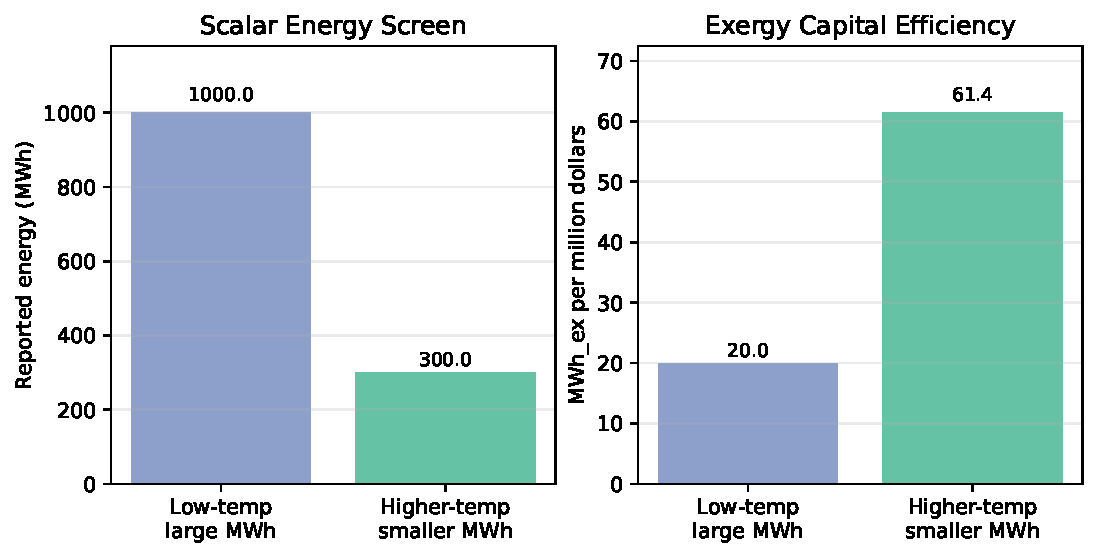
\includegraphics[width=0.82\linewidth]{ece_comparison.pdf}
\caption{Illustrative comparison showing how scalar MWh screening can rank a large low-grade project above a smaller high-grade project, while ECE reverses the ranking on a work-potential basis. The examples are 1{,}000 MWh at $\fx=0.04$ (40 \texttt{MWh\_ex}; 20 \texttt{MWh\_ex} per million dollars) and 300 MWh at $\fx=0.307$ (92.1 \texttt{MWh\_ex}; 61.4 \texttt{MWh\_ex} per million dollars).}
\label{fig:ece_comparison}
\end{figure}

Suppose Project 1 recovers 1,000 MWh of low-temperature heat at $\fx=0.04$ for 2 million dollars. It yields 40 MWh\_ex, or 20 MWh\_ex per million dollars. Project 2 recovers 300 MWh of higher-temperature heat at $\fx=0.307$ for 1.5 million dollars. It yields 92.1 MWh\_ex, or 61.4 MWh\_ex per million dollars. Scalar MWh screening favors Project 1. ECE favors Project 2. The final investment decision still depends on demand, siting, utilization, cost, emissions, risk, and alternatives, but ECE surfaces the thermodynamic opportunity that scalar accounting hides.

\section{Optional Diagnostics: Exergy Loss Angle}

\subsection{Definition and relationship to second-law efficiency}

Before defining the angle, two implementation caveats are important. First, the angle is a display and diagnostic coordinate, not a new state variable. Second, it should be computed from synchronized exergy inputs and outputs over a declared interval; otherwise a dashboard can display a precise-looking angle assembled from asynchronous measurements.

Second-law efficiency is the standard process metric:
\begin{equation}
\eta_X=\frac{X_{\mathrm{useful,out}}}{X_{\mathrm{in}}}.
\end{equation}
For this diagnostic, the non-retained useful work potential over the declared boundary and interval is
\begin{equation}
X_{\mathrm{lost}}=X_{\mathrm{in}}-X_{\mathrm{useful,out}}.
\end{equation}
Here $X_{\mathrm{lost}}$ is a diagnostic residual. It may include exergy destroyed by irreversibility, exergy rejected to the environment, or residual work potential that is not recovered at the declared boundary. It should not automatically be equated with $X_{\mathrm{dest}}=T_0S_{\mathrm{gen}}$ unless a full process balance shows that the residual is thermodynamic destruction.

The Exergy Loss Angle is defined as
\begin{equation}
\thetaloss=\operatorname{atan2}(X_{\mathrm{lost}},X_{\mathrm{useful,out}}).
\end{equation}
The two-argument form is intentional because it handles the zero-output boundary correctly. If $X_{\mathrm{useful,out}}=0$ and $X_{\mathrm{lost}}>0$, a control system should report $\thetaloss=90^{\circ}$, or $\pi/2$ radians, rather than divide by zero or return an error. If both $X_{\mathrm{lost}}=0$ and $X_{\mathrm{useful,out}}=0$, the angle is physically undefined and should be reported as null rather than imputed. For $0<X_{\mathrm{useful,out}}\le X_{\mathrm{in}}$, this can be written in terms of second-law efficiency:
\begin{equation}
\thetaloss=\tan^{-1}\left(\frac{1-\eta_X}{\eta_X}\right).
\end{equation}
The inverse relationship is
\begin{equation}
\eta_X=\frac{1}{1+\tan \thetaloss}.
\end{equation}

The Exergy Loss Angle is therefore not a new thermodynamic property. It is a geometric transformation of second-law efficiency. Its contribution is visual ergonomics and cognitive framing. It maps retained useful work potential to the horizontal axis and non-retained work potential to the vertical axis. A reversible process has $X_{\mathrm{lost}}=0$ and $\thetaloss=0^{\circ}$. A process that retains almost no useful exergy approaches $90^{\circ}$, and a complete dump with nonzero input is reported at the $90^{\circ}$ boundary.

\subsection{Why use an angle?}

Efficiency metrics can visually compress severe degradation. The difference between $\eta_X=0.02$ and $\eta_X=0.06$ can look like a small movement near zero on a conventional efficiency scale, even though the second process retains three times as much useful exergy as the first. The angular representation expands the high-loss region into a bounded visual space from $0^{\circ}$ to $90^{\circ}$. It is not more fundamental than $\eta_X$. It is often easier to scan.

For example:
\begin{center}
\begin{tabular}{@{}ccc@{}}
\toprule
$\eta_X$ & $X_{\mathrm{lost}}/X_{\mathrm{useful,out}}$ & $\thetaloss$ \\
\midrule
0.93 & 0.075 & $4.3^{\circ}$ \\
0.83 & 0.205 & $11.6^{\circ}$ \\
0.50 & 1.0 & $45.0^{\circ}$ \\
0.192 & 4.208 & $76.6^{\circ}$ \\
0.064 & 14.625 & $86.1^{\circ}$ \\
0.020 & 49.000 & $88.8^{\circ}$ \\
\bottomrule
\end{tabular}
\end{center}
The angle makes the distinction between moderate degradation and catastrophic degradation visually immediate. A dashboard can show a near-horizontal process line for efficient retention and a steep line for severe destruction. The information-design rationale is that angular displays expand the visually compressed high-loss region of the efficiency scale into a bounded coordinate that operators can scan quickly, especially when trends and thresholds matter.

\begin{figure}[H]
\centering
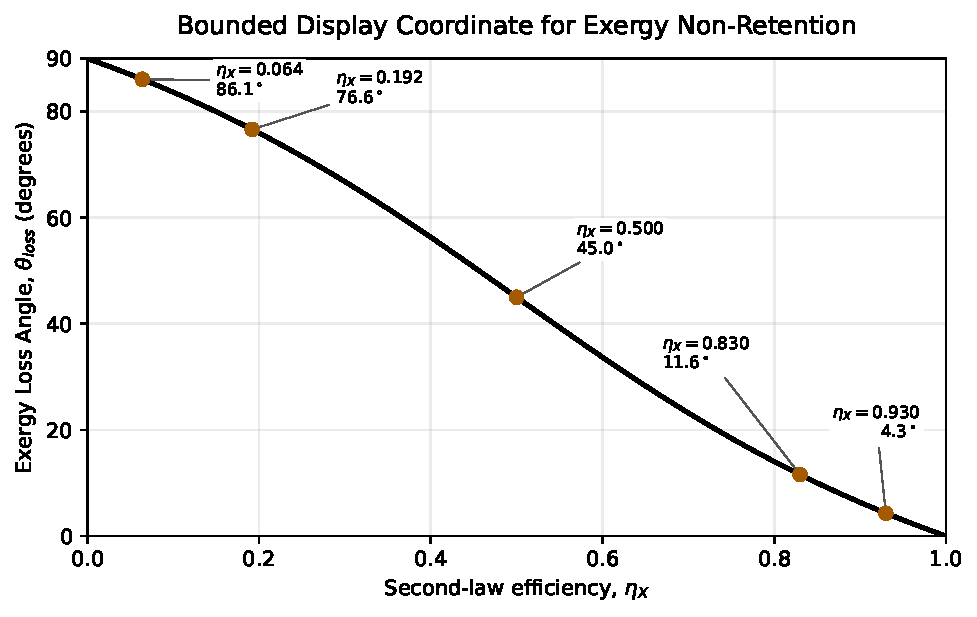
\includegraphics[width=0.82\linewidth]{theta_loss_mapping.pdf}
\caption{Mapping from second-law efficiency to Exergy Loss Angle. The transformation does not add new physics; it changes the visual coordinate used for diagnostics.}
\label{fig:theta_loss_mapping}
\end{figure}

\subsection{Visual grammar}

The framework supports a simple visual grammar:

\begin{table}[H]
\centering
\caption{Visual grammar for typed energy and Exergy Loss Angle displays.}
\begin{tabularx}{\linewidth}{@{}p{0.25\linewidth}X@{}}
\toprule
Visual element & Meaning \\
\midrule
Flat bar & Static stream. The bar represents a reported energy quantity after multiplication by $\fx$. \\
Area of bar & Accessible work potential, $\XA=E\fx$. \\
Sloped process line & Retention of useful output exergy relative to non-retained work potential. \\
Angle of process line & Severity of exergy loss or non-retention, $\thetaloss$. \\
Stacked bars & Multi-carrier portfolio expressed on a comparable MWh\_ex axis. \\
Color or line type & Optional encoding for carrier family, tier, or uncertainty. \\
\bottomrule
\end{tabularx}
\end{table}

The grammar should avoid implying more precision than the data support. A F1 lookup factor should not be displayed with the same confidence as a F4 audit unless the graphic visibly encodes tier or uncertainty. The angle is a display layer on top of a declared calculation.

\subsection{Illustrative angle bands}

For operational dashboards, angle bands may be useful as reference points. The bands below are illustrative only. They are not universal normative thresholds because acceptable loss depends on service, cost, infrastructure, safety, carbon intensity, and alternatives.

\begin{table}[H]
\centering
\caption{Illustrative Exergy Loss Angle bands.}
\begin{tabularx}{0.9\linewidth}{@{}p{0.22\linewidth}p{0.18\linewidth}X@{}}
\toprule
Band & Approximate angle & Interpretation \\
\midrule
Low loss & $0^{\circ}$ to $15^{\circ}$ & High retention of accessible work potential. \\
Moderate loss & $15^{\circ}$ to $45^{\circ}$ & Noticeable degradation; check whether the service justifies it. \\
High loss & $45^{\circ}$ to $75^{\circ}$ & Severe degradation; evaluate matching, cascading, or technology substitution. \\
Extreme loss & $75^{\circ}$ to $90^{\circ}$ & Most accessible work potential is lost or degraded; strong diagnostic alarm unless the service has no better pathway. \\
\bottomrule
\end{tabularx}
\end{table}

\subsection{Loss Angle Velocity}

The time derivative of the Exergy Loss Angle is the Loss Angle Velocity. Because derivatives amplify noise, the calculation rule must be declared before the value is interpreted. In industrial historian systems, $\Delta t$ should represent a fixed, normalized calculation window, such as synchronized 15-minute averages, not raw sequential polling intervals. Temperature, pressure, flow, and composition signals should be resampled or aggregated onto the same time base before $\omegaloss$ is computed; otherwise timestamp jitter and sensor polling latency can create artificial spikes.

With that synchronized window defined,
\begin{equation}
\omegaloss=\frac{d\thetaloss}{dt}.
\end{equation}
In discrete data,
\begin{equation}
\omegaloss(t_k)\approx \frac{\thetaloss(t_k)-\thetaloss(t_{k-1})}{\Delta t}.
\end{equation}
The units are degrees per hour, degrees per day, or radians per unit time depending on the dashboard. Positive $\omegaloss$ means worsening exergy retention. Negative $\omegaloss$ means improving retention. F3 and F4 implementations should declare smoothing, filtering, deadbands, and missing-data rules. In industrial monitoring, $\omegaloss$ is most useful as a trend and anomaly indicator, not as a standalone proof of failure.

\section{Illustrative Applications and Screening Examples}

The following cases demonstrate how the framework changes interpretation while preserving existing energy quantities. They use rounded engineering figures for illustration. The empirical demonstration is separated into Section 9 so that illustrative examples are not confused with measured operational results. In each case, the public token is compact, while the fidelity tier and metadata determine audit strength.

\subsection*{Case A: Plant operator thermodynamic mismatch log}

A plant operator managing boilers, steam headers, condensate return, heat exchangers, and waste-heat loops often sees energy quantities as separate instrumentation streams. The proposed reporting layer converts those streams into a common work-potential log:

\begin{center}
\begin{tabular}{@{}lll@{}}
\toprule
Stream & Conventional report & Typed report \\
\midrule
Electric drive input & 50 MWh & \texttt{50 MWh\_e, fx = 1.0} \\
Steam header heat & 100 MWh & \texttt{100 MWh\_th, fx = 0.307 [Th = 150C]} \\
Warm water return & 80 MWh & \texttt{80 MWh\_th, fx = 0.064 [Th = 40C]} \\
Methane fuel & 500 MWh & \texttt{500 MWh\_HHV\_CH4, fx = 0.93} \\
\bottomrule
\end{tabular}
\end{center}

The operator can now distinguish energy throughput from thermodynamic grade. A 100 MWh steam header at $150\degC$ carries approximately 30.7 MWh\_ex. An 80 MWh warm-water return at $40\degC$ carries about 5.1 MWh\_ex relative to the same sink. The scalar report sees the warm-water loop as a large resource. The typed report sees a low-grade resource that must be matched to a low-grade demand or upgraded.

The mismatch log can be expressed as $\Delta \fx$ between supply and service. If a high-temperature source with $\fx=0.307$ is routed to a service requiring $\fx=0.064$, the oversupplied work-potential grade is $0.243$ per MWh of matched heat. If no cascade exists, that mismatch becomes a loss candidate. This is not a condemnation of the heat service. It is a diagnostic for whether the plant is using too much grade for too little thermodynamic requirement.

\subsection*{Case B: District heating network}

District heating is an ideal early domain because temperatures and heat flows are already measured. Consider a network delivering 1.00 MWh of heat demand composed of 0.40 MWh at $80\degC$ and 0.60 MWh at $40\degC$, both relative to a $20\degC$ sink. The factors are
\begin{equation}
\fx(80\degC)=0.170,
\end{equation}
\begin{equation}
\fx(40\degC)=0.064.
\end{equation}
If the whole network is supplied uniformly at the higher grade, the report is
\begin{equation}
\texttt{1.00 MWh\_th, fx = 0.170},
\end{equation}
with 0.170 MWh\_ex supplied. If the service portfolio is reported by grade, the demand is
\begin{equation}
\texttt{0.40 MWh\_th, fx = 0.170}+\texttt{0.60 MWh\_th, fx = 0.064},
\end{equation}
with service exergy
\begin{equation}
X_d=(0.40)(0.170)+(0.60)(0.064)=0.106\ \text{\texttt{MWh\_ex}}.
\end{equation}
The hidden mismatch is about 0.064 MWh\_ex.

In F3 operation, $\fx(t)$ can be computed continuously from supply and return temperatures. A tariff or dispatch optimizer can then reward lower return temperatures, cascading, and heat-pump integration not merely because they save heat quantity, but because they preserve or recover work-potential grade.


\subsection*{Case C: Industrial waste-heat recovery}

Industrial waste heat is commonly screened by total MWh available. This can mislead capital allocation. Compare two candidate streams:
\begin{center}
\begin{tabular}{@{}lccc@{}}
\toprule
Stream & Energy & $\fx$ & Accessible exergy \\
\midrule
High-temperature exhaust & \texttt{300 MWh\_th} & 0.307 & 92.1 MWh\_ex \\
Ultra-low-temperature loop & \texttt{1000 MWh\_th} & 0.040 & 40.0 MWh\_ex \\
\bottomrule
\end{tabular}
\end{center}
The scalar report ranks the second stream as more than three times larger. The exergy-aware report ranks the first stream at more than twice the accessible work potential. Capital screening should not ignore location, capture cost, heat exchanger economics, operating hours, fouling, or service match. But the typed report prevents the most basic error: confusing large heat quantity with high recoverable utility.

If the high-temperature stream is recovered through a process that delivers 60 MWh\_ex useful output from 92.1 MWh\_ex input, then $\eta_X=0.651$ and $\theta_{\mathrm{loss}}=28.2^{\circ}$. If the ultra-low-temperature loop requires substantial parasitic energy and delivers only 10 MWh\_ex useful output from 40 MWh\_ex accessible input, then $\eta_X=0.25$ and $\theta_{\mathrm{loss}}=71.6^{\circ}$. The angle reveals that the larger scalar-MWh project may be a worse thermodynamic conversion opportunity.

\subsection*{Case D: Electrification, resistance heating, and heat pumps}

Consider a demand for 1.00 MWh of heat delivered at $40\degC$ to a sink at $20\degC$. The service Exergy Factor is
\begin{equation}
f_{X,d}=1-\frac{293.15}{313.15}=0.064.
\end{equation}
The demanded useful exergy service is therefore
\begin{equation}
X_d=(1.00)(0.064)=0.064\ \text{\texttt{MWh\_ex}}.
\end{equation}

A resistance heater consumes approximately 1.00 MWh of electricity, or 1.00 MWh\_ex input, to deliver the heat service. Its second-law efficiency relative to the low-temperature heat service is therefore
\begin{equation}
\eta_X=\frac{0.064}{1.00}=0.064,
\end{equation}
and its Exergy Loss Angle is
\begin{equation}
\thetaloss=\tan^{-1}\left(\frac{1-0.064}{0.064}\right)=86.1^{\circ}.
\end{equation}

A heat pump with COP = 3 consumes 0.333 MWh of electricity to deliver the same 1.00 MWh of heat. Its second-law efficiency is
\begin{equation}
\eta_X=\frac{0.064}{0.333}=0.192,
\end{equation}
with
\begin{equation}
\thetaloss=76.6^{\circ}.
\end{equation}
Both devices deliver the same first-law heat quantity. The heat pump consumes much less high-grade input exergy and shifts the loss angle downward. The angle remains high because low-temperature heat is a low-exergy service and real heat pumps are irreversible. The key point is that the framework makes the difference visible in one line of reporting.

\subsection*{Case E: Stationary storage systems}

Storage assets are often compared by rated MWh. That comparison is incomplete because the stored carrier matters. A battery, a hot-water tank, and hydrogen storage may all be reported as 1 MWh, but their accessible work potential differs.

\begin{center}
\begin{tabular}{@{}lccc@{}}
\toprule
Storage asset & Typed report & $\fx$ & MWh\_ex per MWh \\
\midrule
Battery & \texttt{1 MWh\_e} & 1.0 & 1.0 \\
Hot-water storage, $80\degC$ & \texttt{1 MWh\_th} & 0.170 & 0.170 \\
Hot-water storage, $40\degC$ & \texttt{1 MWh\_th} & 0.064 & 0.064 \\
Hydrogen, HHV & \texttt{1 MWh\_HHV\_H2} & 0.83 & 0.83 \\
Methane, HHV & \texttt{1 MWh\_HHV\_CH4} & 0.93 & 0.93 \\
\bottomrule
\end{tabular}
\end{center}
This does not mean batteries are always better than thermal storage. A hot-water tank can be excellent if the demand is hot water or space heating. The table means that storage valuation must specify the service. A low-$\fx$ storage asset can be the best match for a low-$\fx$ demand, while a high-$\fx$ storage asset should be reserved for services requiring high work potential.

\subsection*{Case F: Investor screening}

Case F applies the Exergy Capital Efficiency diagnostic defined in Section 6.4. A scalar investment screen may rank a project by MWh recovered, while an exergy-aware screen ranks by MWh\_ex delivered per dollar. In the example used above, a 1,000 MWh low-temperature recovery project delivers only 40 MWh\_ex, while a 300 MWh higher-temperature project delivers 92.1 MWh\_ex. The exergy screen does not make the investment decision by itself, but it prevents capital allocators from mistaking large low-grade heat quantity for high thermodynamic utility.

\section{Empirical Demonstration: F3 District-Heating Implementation}

\subsection{Data and method}

A proposed reporting framework becomes more credible when it can be applied directly to operational telemetry without adding new sensors. This paper therefore analyzes the public XAI4HEAT GitHub repository at commit \texttt{fc7ee9a} \cite{xai4heatgithub}, using the processed files \texttt{xai4heat\_2024-25\_L4.csv}, \texttt{xai4heat\_2024-25\_L12.csv}, \texttt{xai4heat\_2024-25\_L17.csv}, and \texttt{xai4heat\_2024-25\_L22.csv}. The repository is associated with the XAI4HEAT SCADA dataset and its Data in Brief description \cite{xai4heat2024,cvetkovic2025}. Each file is a 15-minute district-heating time series spanning 17 November 2024 through 31 March 2025. The repository also contains raw SCADA files for L4, L8, L12, L17, and L22 with a shared structure containing timestamps, ambient temperature, primary and secondary supply and return temperatures, and meter fields, confirming that the F3 computation pathway generalizes across substations.

For each processed interval, the base F3 reporting factor was computed from measured primary supply temperature and measured ambient temperature:
\begin{equation}
f_{X,k}^{\mathrm{sup}}=1-\frac{T_{\mathrm{amb},k}}{T_{\mathrm{sup,prim},k}}=1-\frac{t_{\mathrm{amb},k}+273.15}{t_{\mathrm{sup,prim},k}+273.15}.
\end{equation}
This supply-temperature Carnot factor is intentionally a reporting approximation. It is appropriate for demonstrating F3 interval tagging from measured telemetry, but a district-heating water stream is not a constant-temperature heat source. The processed files include primary and secondary return temperatures, so the analysis also computes a supply-return integrated water-stream factor:
\begin{equation}
f_{X,k}^{\mathrm{int}}=1-\frac{T_{0,k}\ln(T_{\mathrm{sup},k}/T_{\mathrm{ret},k})}{T_{\mathrm{sup},k}-T_{\mathrm{ret},k}},
\end{equation}
which is the exergy fraction of sensible heat delivered as water cools from supply to return temperature under a constant heat-capacity approximation. A third sensitivity treats the primary return temperature as the operational sink:
\begin{equation}
f_{X,k}^{\mathrm{return}}=1-\frac{T_{\mathrm{ret,prim},k}}{T_{\mathrm{sup,prim},k}}.
\end{equation}
These alternatives do not replace the base F3 tag; they show how the reported factor changes when the method boundary moves toward a fuller stream description.

The processed files also contain a nonnegative thermal-delivery field, \texttt{qizm}, which is used here as the interval weight for exergy-weighted averaging. Across four substations and 51{,}592 valid 15-minute intervals, the \texttt{qizm}-weighted portfolio Exergy Factor is 0.216 with the measured ambient sink. If the same intervals are reported under a fixed default sink of $20\degC$, the weighted factor is 0.173. The dynamic-sink treatment therefore changes the seasonal portfolio factor by 0.044 in absolute terms, or about 25\% relative to the fixed-sink value.

\subsection{Results}

During the cold event centered on 20 February 2025, dynamic interval Exergy Factors peaked between 0.277 and 0.286 across the processed substations. These results are operationally important because they show that the same heat network can move across materially different quality states without changing carrier identity. A flat \texttt{MWh\_th} thermal-energy total cannot reveal that shift; an F3 stream tag can.

\begin{table}[H]
\centering
\small
\caption{Empirical F3 summary for XAI4HEAT processed 2024--2025 season files. Dynamic factors use measured ambient temperature as sink; fixed factors use $T_0=20\degC$.}
\label{tab:xai4heat_summary}
\begin{tabular}{@{}lrrrrr@{}}
\toprule
Station & Intervals & $f_X$ dynamic & $f_X$ fixed & $\Delta f_X$ & Peak $f_X$ \\
\midrule
L4 & 12{,}898 & 0.217 & 0.172 & 0.045 & 0.286 \\
L12 & 12{,}898 & 0.219 & 0.174 & 0.044 & 0.284 \\
L17 & 12{,}898 & 0.217 & 0.173 & 0.044 & 0.284 \\
L22 & 12{,}898 & 0.212 & 0.172 & 0.041 & 0.277 \\
Portfolio & 51{,}592 & 0.216 & 0.173 & 0.044 & 0.286 \\
\bottomrule
\end{tabular}
\end{table}

\begin{table}[H]
\centering
\small
\caption{Thermal-model sensitivity for the XAI4HEAT portfolio. Values are \texttt{qizm}-weighted over the processed substations L4, L12, L17, and L22.}
\label{tab:xai4heat_sensitivity}
\begin{tabularx}{\linewidth}{@{}p{0.30\linewidth}p{0.17\linewidth}p{0.17\linewidth}X@{}}
\toprule
Model & Portfolio $\fx$ & Valid intervals & Purpose \\
\midrule
Primary supply, ambient sink & 0.216 & 51{,}592 & Base F3 reporting approximation, $1-T_{\mathrm{amb}}/T_{\mathrm{sup,prim}}$. \\
Primary supply-return integration & 0.172 & 46{,}434 & More thermodynamically detailed water-stream estimate using primary supply and return temperatures. \\
Secondary supply-return integration & 0.125 & 49{,}314 & Service-side proxy using secondary supply and return temperatures where available and thermodynamically distinguishable from ambient. \\
Primary return as sink & 0.106 & 46{,}438 & Operational sink sensitivity, $1-T_{\mathrm{ret,prim}}/T_{\mathrm{sup,prim}}$, restricted to intervals with supply no colder than return. \\
Primary supply, fixed $20\degC$ sink & 0.173 & 51{,}592 & Comparable-reporting reference using the paper's default sink. \\
\bottomrule
\end{tabularx}
\end{table}

The sensitivity table narrows the empirical claim. The XAI4HEAT pass demonstrates that the interface can be computed from real telemetry and that sink and method choices materially change reported quality. It does not validate the full Carrier Registry, chemical-carrier treatment, Exergy Capital Efficiency, or Exergy Loss Angle. Instead, it shows why the Fidelity Tier, \texttt{method\_id}, boundary, and reference fields are required: the same \texttt{MWh\_th} interval can reasonably carry different $\fx$ values under different declared thermal models. The primary integrated model excludes 5{,}158 intervals with missing or invalid supply-return conditions; the primary return-sink model accepts the four equilibrium intervals at $\fx=0$ and excludes the remaining 5{,}154 reversed intervals. The secondary integrated proxy excludes 2{,}278 intervals, including 71 zero-delivery intervals whose logarithmic-mean stream temperature does not exceed ambient; reporting any of these reversed states as negative heat-stream factors would violate the declared distinguishability rule.

\begin{table}[H]
\centering
\small
\caption{Temperature-only uncertainty sensitivity for the XAI4HEAT portfolio. Ranges assume symmetric $\pm 0.5\degC$ uncertainty on measured temperature fields; no \texttt{qizm} meter uncertainty is propagated because meter specifications were not available in the processed files.}
\label{tab:xai4heat_uncertainty}
\begin{tabularx}{\linewidth}{@{}p{0.34\linewidth}p{0.16\linewidth}p{0.20\linewidth}X@{}}
\toprule
Model & Base $\fx$ & Perturbed range & Approx. $|\Delta \fx|$ \\
\midrule
Primary supply, ambient sink & 0.216 & 0.214--0.219 & 0.003 \\
Primary supply-return integration & 0.172 & 0.169--0.175 & 0.003 \\
Secondary supply-return integration & 0.125 & 0.122--0.128 & 0.003 \\
Primary return as sink & 0.106 & 0.103--0.108 & 0.003 \\
Primary supply, fixed $20\degC$ sink & 0.173 & 0.171--0.174 & 0.001 \\
\bottomrule
\end{tabularx}
\end{table}

This uncertainty treatment is intentionally modest. It is not a substitute for a metrologically complete F4 uncertainty propagation with sensor calibration records, meter uncertainty, timestamp uncertainty, and missing-data imputation. It is included to make the F3 demonstration auditable: under a simple $\pm 0.5\degC$ temperature perturbation, the temperature-only uncertainty is much smaller than the method and reference-sink differences reported in Table \ref{tab:xai4heat_sensitivity}.

Figure \ref{fig:f3_backcast} shows the resulting empirical F3 demonstration. The top panel reports daily \texttt{qizm}-weighted Exergy Factors for the full season across the processed substations, comparing the dynamic ambient sink with a fixed $20\degC$ sink. The bottom panel zooms into the February cold event and shows how the portfolio Exergy Factor rises as supply temperature increases and ambient temperature falls.

\begin{figure}[H]
\centering
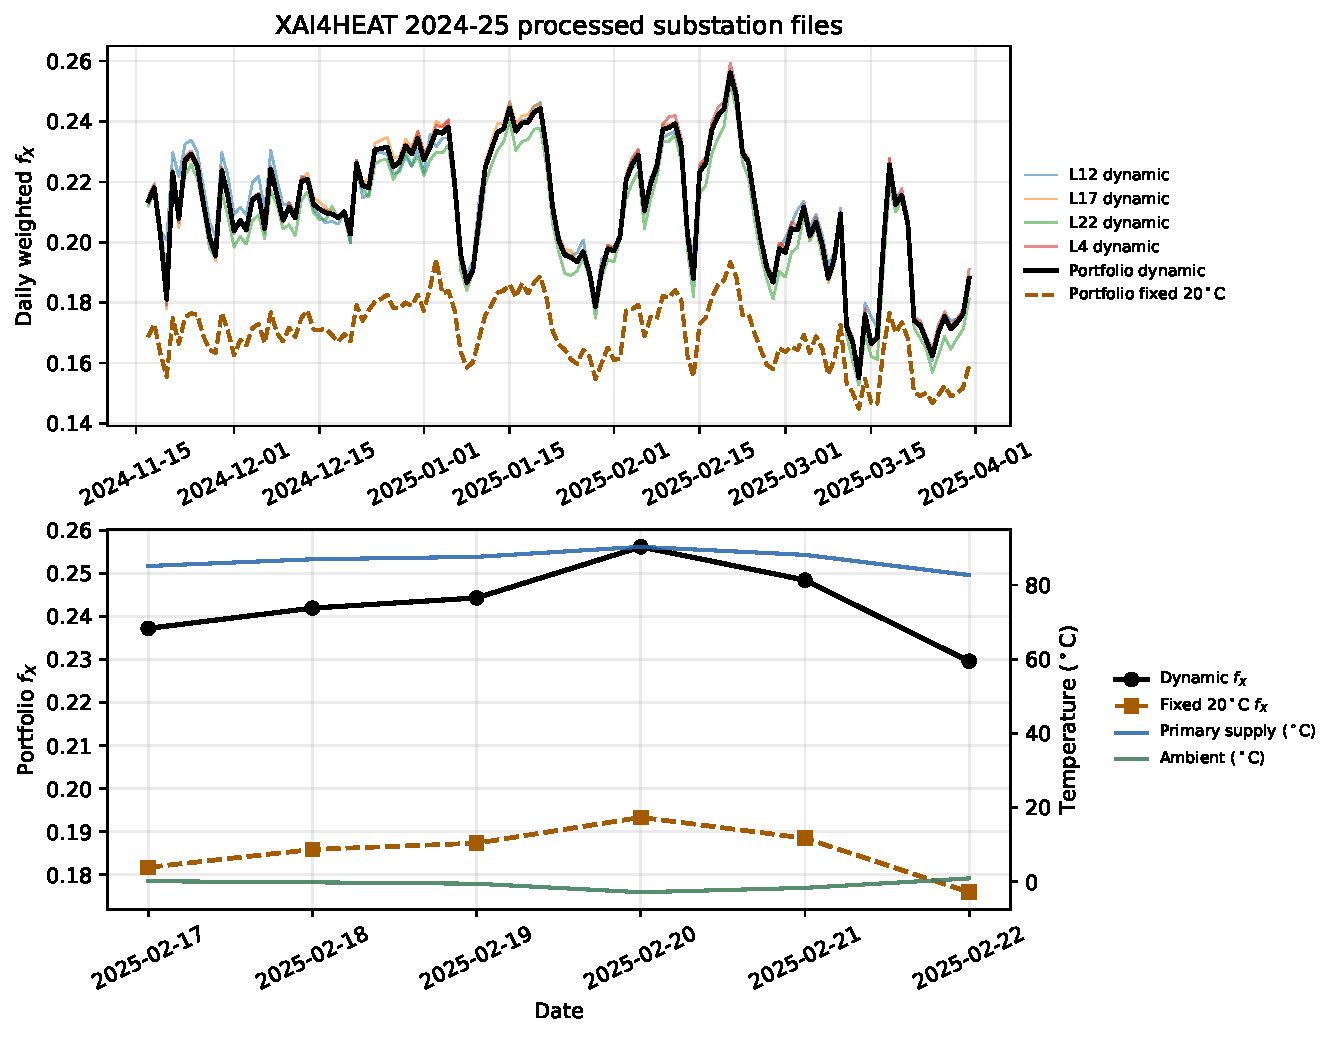
\includegraphics[width=0.90\linewidth]{f3_district_heat_backcast.pdf}
\caption{Empirical F3 demonstration using processed XAI4HEAT district-heating data. Top: daily \texttt{qizm}-weighted Exergy Factors for the 2024--2025 heating season across processed substations L4, L12, L17, and L22. Bottom: cold-snap zoom showing portfolio primary supply temperature, ambient temperature, and the resulting dynamic $f_X$.}
\label{fig:f3_backcast}
\end{figure}

\subsection{Interpretation}

This empirical proof-of-implementation materially strengthens the framework, but its scope is deliberately limited. It demonstrates that the typed reporting token can be computed from operational telemetry, that the F3 tier survives real time-series data, and that reference-sink and method choices have measurable effects on reported thermodynamic quality. A larger follow-on validation study should reconcile the processed and raw meter fields, extend the analysis to the repository's raw L8 data, compare against full F4 stream balances, and publish a full reproducible workflow.

\section{Epistemological Boundaries and Institutional Friction}

\subsection{What the framework does not claim}

The framework is an accounting and reporting proposal, not a new thermodynamic law. It does not claim that Exergy Factor is intrinsic to matter. It does not claim that a single scalar captures every detail of a non-equilibrium system. It does not replace plant design, equipment sizing, detailed chemical calculations, phase-equilibrium modeling, life-cycle assessment, carbon accounting, economic dispatch, reliability analysis, or localized COP modeling. It does not make reference-state dependence disappear.

The claim is narrower and more practical: when institutions already report energy quantities, those quantities should carry enough carrier and Exergy Factor information to avoid false comparability across unlike work-potential grades. The public token is minimal, but the Fidelity Tier and metadata determine what the token can be used for.

\subsection{Reference dependence is managed, not eliminated}

Because exergy is relational, every $\fx$ value depends on a reference. The framework manages this in three ways. First, it recommends default references for comparability. Second, it allows local or dynamic references for operational control. Third, it requires metadata at the appropriate tier. A reviewer should reject any claim that reports $\fx$ without carrier, basis, boundary, or reference context when those details materially affect the value.

\subsection{Data resolution and uncertainty}

Thermal reporting requires temperature resolution. Chemical reporting requires basis and composition. Pressure and compressed-gas reporting require pressure, volume, and system boundary. Dynamic operation requires interval rules, sensor quality, outlier handling, and missing-data governance. These are implementation burdens, but they are not unique to exergy. Carbon accounting, electricity settlement, weather-normalized savings, and IPMVP baselines all require data governance. The proposed Fidelity Tiers exist so a report can state how strong its data foundation is.

\subsection{Data readiness}

The XAI4HEAT demonstration shows that some operational datasets already contain the fields needed for dynamic Exergy Factor reporting: energy or thermal-delivery increments, temperatures, timestamps, and a plausible reference signal. Other public datasets show a complementary readiness pattern. The Foundational Industry Energy Dataset compiles unit-level industrial facility information, including unit type, fuel type, design capacity, and energy estimates from public U.S. EPA sources \cite{fiedgithub}. It does not by itself provide enough temperature-grade information to compute stream-specific Exergy Factors, but it shows that industrial data systems already have facility and unit identifiers to which carrier, basis, reference, and fidelity metadata could be attached.

This distinction matters. The proposed framework does not require every dataset to become a full exergy audit. It requires datasets to stop treating first-law energy quantities as self-describing. Where a dataset has enough temperature, pressure, composition, or service-boundary information, it can support F2 or F3 factors directly. Where it does not, it can still expose the missing field explicitly and avoid implying false comparability.

\subsection{Interoperability with industrial systems}

The interface layer is deliberately compatible with existing data infrastructure. The underscore-delimited token can be used in SCADA tags, historian variables, SQL columns, CSV headers, MQTT Sparkplug B metrics, JSON payloads, regulatory forms, invoices, and dashboards without changing the physical meter. Examples include:

\begin{verbatim}
site.loop4.energy_token = "MWh_th"
site.loop4.fx = 0.170
site.loop4.fx_tier = "F2"
site.loop4.metadata = "Th = 80C; T0 = 20C"
\end{verbatim}

or, in a structured payload:
\begin{verbatim}
{
  "stream_id": "loop4",
  "energy": 100.0,
  "unit": "MWh_th",
  "fx": 0.170,
  "tier": "F2",
  "method_id": "thermal.carnot.constant_temperature.v1",
  "reference": {"T0_C": 20.0, "p0_kPa": 101.325},
  "boundary": "district_heat_primary_supply",
  "basis": "thermal_delivery",
  "timestamp": "2026-05-01T00:00:00Z",
  "uncertainty": {"fx_abs": 0.005},
  "data_quality_flag": "measured",
  "carrier_registry_version": "0.1",
  "source": {"Th_C": 80.0}
}
\end{verbatim}

The point is not to force a new metering stack. It is to add fields to the systems that already store energy quantities. Adoption should begin as a supplemental column, not as a replacement architecture.

\subsection{Institutional adoption path}

Concretely, candidate institutional homes include ISO/TC 301 for energy management systems, ISO/TC 207 for life-cycle assessment interfaces, IEC TC 8 for system aspects of electrical energy supply, and an IEEE Power and Energy Society working group for machine-readable energy-quality tags. The most immediate first movers are district-heating operators already collecting supply and return temperatures, as demonstrated by XAI4HEAT, and industrial sites already maintaining ISO 50001 energy performance indicators. Early pilots are especially plausible in district-heating utilities in Denmark, Sweden, Serbia, or other regions with mature temperature telemetry and active network optimization programs.

The fastest path is targeted pilots. District heating and cooling networks can compute $\fx(t)$ from existing supply and return temperatures. Industrial sites can screen waste heat by MWh\_ex rather than MWh. Hydrogen and synthetic-fuel policy frameworks can declare HHV or LHV basis explicitly. ISO 50001 programs can test Exergy Factor as a supplemental performance indicator. IPMVP reports can include both $\Delta E$ and $\Delta X_A$:
\begin{equation}
\Delta E=E_{\mathrm{baseline}}-E_{\mathrm{post}},
\end{equation}
\begin{equation}
\Delta X_A=(\fx E)_{\mathrm{baseline}}-(\fx E)_{\mathrm{post}}.
\end{equation}
Life-cycle inventories can attach carrier and Exergy Factor attributes to energy flows. Markets can settle heat products with both MWh and MWh\_ex attributes. None of these pilots requires abandoning existing accounting. They require adding a thermodynamic quality layer.

\subsection{Social and institutional friction}

The greatest barrier may be that scalar energy reporting is familiar. Institutions prefer metrics that are additive, stable, and easy to compare. Exergy is relational, which makes it more precise but operationally less comfortable. The two-layer architecture is designed to meet that reality. The physics layer protects rigor. The interface layer protects adoption. The Fidelity Tiers protect transparency. Optional diagnostics such as the Exergy Loss Angle support interpretability when a dashboard needs them.

The proposed protocol should therefore be introduced as an upgrade path, not as a critique of every existing metric. MWh remains useful. Cost remains useful. Emissions remain useful. Life-cycle impacts remain useful. The missing field is work potential. Adding it makes existing metrics more informative.

\section{Conclusion}

This paper proposes a single practical change to energy reporting: every reported energy quantity should carry an Exergy Factor. The result is a typed two-number framework, $(E_{\mathrm{carrier}},\fx)$, that preserves conventional first-law quantities while attaching a second-law quality field. Electricity, heat, fuels, storage assets, pressure systems, and mechanical work can continue to be reported in familiar units, but those units no longer travel without carrier and work-potential context.

The physics layer provides the justification. Accessible exergy is relational. The exergy voltage, $\Delta\Phi_A^{(C)}=dX_A/dC$, generalizes voltage-like potentials across carriers. The universal flow law, $\XdotA=\dot{C}\Delta\Phi_A^{(C)}=\fx\dot{E}$, links carrier current, accessible potential, and normalized reporting. The unified carrier matrix shows why a single public interface can be defensible without pretending that all carriers are physically identical.

The interface layer provides the adoption path. Typed-energy notation, a Carrier Registry, bracket metadata, a declare-once basis block, and Fidelity Tiers F0 through F4 allow the same framework to function in a spreadsheet, a plant historian, a district-energy control room, a fuel policy report, or a full engineering audit. The Thermodynamic Honesty Rule prevents the simplicity of the front end from becoming a false claim of intrinsic scalar quality.

The diagnostic layer provides operational meaning. Supply and demand should be matched in both quantity and Exergy Factor. Stream quality must be separated from process irreversibility. The Exergy Loss Angle converts second-law efficiency into a bounded angular display coordinate for visual diagnostics, while the Loss Angle Velocity supplies a trend signal for degradation and predictive maintenance. These diagnostics are secondary to the proposed reporting protocol, but they show how the quality field can be used once it exists.

The empirical demonstration shows that the framework is not merely notational. Public XAI4HEAT district-heating data can be converted into F3 interval Exergy Factor records from measured supply temperature, ambient temperature, and thermal-delivery weights. The difference between the dynamic ambient-sink factor, the fixed-reference factor, and the supply-return sensitivity cases is large enough to matter for reporting, dispatch, and benchmarking. Existing datasets already contain much of the required structure; the missing element is a shared thermodynamic quality field.

Energy-transition reporting would benefit from a quality field that distinguishes energy magnitude from accessible work potential. Decarbonization changes the sources of energy, but it does not remove the need to match high-grade resources to high-grade services and low-grade resources to low-grade services. Low-grade heat can be ignored because it looks small in market terms or overvalued because it looks large in scalar MWh. Storage, fuels, industrial heat, district energy, and electrification all require clearer accounting of what reported energy can actually do.

Cleaner energy carriers still need clearer accounting. The proposed $(E_{\mathrm{carrier}},\fx)$ framework is a minimum practical upgrade for making useful work potential visible alongside energy quantity.

\appendix

\section{Quick Start Implementation Cheat Sheet}

This appendix condenses the reporting protocol into an implementation checklist for data teams, plant engineers, and reviewers. It is not a substitute for the Fidelity Tiers; it is the minimum practical pattern for making the framework machine-readable.

\subsection*{A.1 Public token}

Report every energy quantity with a carrier suffix and Exergy Factor:
\begin{center}
\begin{tabularx}{\linewidth}{@{}>{\ttfamily\footnotesize\raggedright\arraybackslash}p{0.50\linewidth}X@{}}
\toprule
\normalfont Example token & Meaning \\
\midrule
100 MWh\_e, fx = 1.0 & Electricity, work-equivalent at point of use. \\
100 MWh\_th, fx = 0.170 [Th = 80C, T0 = 20C] & Thermal energy at $80\degC$ relative to a $20\degC$ sink. \\
100 MWh\_HHV\_CH4, fx = 0.93 [basis = HHV] & Methane on higher-heating-value basis. \\
\bottomrule
\end{tabularx}
\end{center}

\subsection*{A.2 Minimum fields}

A machine-readable record should carry at least the following fields:
\begin{center}
\begin{tabularx}{0.96\linewidth}{@{}p{0.32\linewidth}p{0.15\linewidth}X@{}}
\toprule
Field & Required & Purpose \\
\midrule
\texttt{stream\_id} & Yes & Stable stream, meter, asset, or interval identifier. \\
\texttt{quantity} & Yes & First-law energy or rate value. \\
\texttt{unit} & Yes & Carrier-aware unit, such as \texttt{MWh\_th} or \texttt{MW\_e}. \\
\texttt{fx} & Yes for F1+ & Exergy Factor at the declared boundary. \\
\texttt{tier} & Yes & Fidelity Tier F0 through F4. \\
\texttt{reference} & Yes for F2+ & Reference sink, pressure, basis, or environment. \\
\texttt{boundary} & Yes for F2+ & Physical or accounting boundary for the reported value. \\
\texttt{basis} & As needed & Energy denominator and table convention. \\
\texttt{method\_id} & Yes for F2+ & Calculation method or model identifier. \\
\texttt{timestamp} & Yes for F3+ & Interval timestamp or validity window. \\
\texttt{uncertainty} & As needed & Reported uncertainty or confidence band. \\
\texttt{data\_quality\_flag} & Yes for F3+ & Missing-data, outlier, sensor-quality, or synchronization flag. \\
\texttt{carrier\_registry\_version} & Yes & Registry version used to parse the suffix; this draft uses \texttt{0.1}. \\
\texttt{metadata} & As needed & Additional temperature, pressure, composition, interval, source, and QA fields. \\
\bottomrule
\end{tabularx}
\end{center}

\subsection*{A.3 Core formulas}

\begin{align}
X_A &= \fx E, \\
\dot{X}_A &= \fx P, \\
f_{X,Q} &= 1-\frac{T_0}{T_h}, \\
\bar{f}_X &= \frac{\int f_X(t)\dot{E}(t)\,dt}{\int \dot{E}(t)\,dt}.
\end{align}
For interval data, replace the integrals with synchronized sums:
\begin{equation}
\bar{f}_X=\frac{\sum_k f_{X,k} E_k}{\sum_k E_k}.
\end{equation}

\subsection*{A.4 Fidelity Tier shortcut}

\begin{center}
\begin{tabularx}{0.92\linewidth}{@{}lX@{}}
\toprule
Tier & Minimum interpretation \\
\midrule
F0 & Scalar legacy reporting only; no Exergy Factor claim. \\
F1 & Presumptive lookup factor; useful for screening only. \\
F2 & Asset-specific factor with declared reference, basis, and boundary. \\
F3 & Dynamic interval factor from synchronized operational telemetry. \\
F4 & Full state-vector audit with engineering-grade exergy balance. \\
\bottomrule
\end{tabularx}
\end{center}

\subsection*{A.5 Conformance checklist}

A conforming report should declare the carrier, basis, reference, boundary, and Fidelity Tier once, then attach \texttt{fx} values to every reported energy quantity covered by that declaration. F3 records should additionally declare interval length, timestamp convention, synchronization method, missing-data rule, and outlier rule. F4 records should declare the full state variables, model assumptions, and balance closure criteria.

\subsection*{A.6 Structured payload}

\begin{verbatim}
{
  "stream_id": "loop4",
  "quantity": 100.0,
  "unit": "MWh_th",
  "fx": 0.170,
  "tier": "F2",
  "method_id": "thermal.carnot.constant_temperature.v1",
  "reference": {"T0_C": 20.0, "p0_kPa": 101.325},
  "boundary": "district_heat_primary_supply",
  "basis": "thermal_delivery",
  "timestamp": "2026-05-01T00:00:00Z",
  "uncertainty": {"fx_abs": 0.005},
  "data_quality_flag": "measured",
  "carrier_registry_version": "0.1",
  "metadata": {"Th_C": 80.0}
}
\end{verbatim}

\section{XAI4HEAT Reproducibility Notes}

This appendix gives the exact reproducibility path for the empirical district-heating demonstration in Section 9. It is intended to make the proof-of-implementation auditable without implying that the demonstration is a full F4 validation study.

\subsection*{B.1 Source repository and files}

The analysis uses the public XAI4HEAT repository at commit \texttt{fc7ee9a} \cite{xai4heatgithub}. The processed files used for Tables \ref{tab:xai4heat_summary}, \ref{tab:xai4heat_sensitivity}, and \ref{tab:xai4heat_uncertainty} are:
\begin{verbatim}
runtime/external/xai4heat/datasets/xai4heat_2024-25_L4.csv
runtime/external/xai4heat/datasets/xai4heat_2024-25_L12.csv
runtime/external/xai4heat/datasets/xai4heat_2024-25_L17.csv
runtime/external/xai4heat/datasets/xai4heat_2024-25_L22.csv
\end{verbatim}

The columns used directly are \texttt{datetime}, \texttt{t\_amb}, \texttt{t\_sup\_prim}, \texttt{t\_ret\_prim}, \texttt{t\_sup\_sec}, \texttt{t\_ret\_sec}, and \texttt{qizm}. The field \texttt{qizm} is treated as a nonnegative interval weight. Negative weights are clipped to zero in the analysis script.

\subsection*{B.2 Reproduction commands}

From the repository root, the demonstration can be reproduced with:
\begin{verbatim}
git clone https://github.com/xai4heat/xai4heat runtime/external/xai4heat
git -C runtime/external/xai4heat checkout fc7ee9a
python -m pip install ".[paper]"
python scripts/analyze_xai4heat.py
python scripts/generate_paper_figures.py
make -C paper pdf
\end{verbatim}

The analysis script accepts an explicit root if the XAI4HEAT clone is stored elsewhere:
\begin{verbatim}
python scripts/analyze_xai4heat.py \
  --xai4heat-root /path/to/xai4heat
\end{verbatim}

\subsection*{B.3 Generated artifacts}

The script \texttt{scripts/analyze\_xai4heat.py} writes the following reproducibility artifacts:
\begin{verbatim}
paper/generated/xai4heat_f3_summary.csv
paper/generated/xai4heat_f3_daily.csv
paper/generated/xai4heat_f3_model_sensitivity.csv
paper/generated/xai4heat_f3_uncertainty.csv
paper/f3_district_heat_backcast.pdf
\end{verbatim}

The published tables and figures map to generated artifacts as follows:
\begin{itemize}
\item Table \ref{tab:xai4heat_summary}: \path{xai4heat_f3_summary.csv}.
\item Table \ref{tab:xai4heat_sensitivity}: \path{xai4heat_f3_model_sensitivity.csv}.
\item Table \ref{tab:xai4heat_uncertainty}: \path{xai4heat_f3_uncertainty.csv}.
\item Figure \ref{fig:f3_backcast}: \path{f3_district_heat_backcast.pdf}.
\end{itemize}
The deterministic figures that do not require XAI4HEAT data are generated by
\path{scripts/generate_paper_figures.py}.

\subsection*{B.4 Calculation rule}

For each valid interval, temperatures are converted from degrees Celsius to kelvin by adding 273.15. The base F3 supply-temperature model is
\begin{equation}
f_{X,k}^{\mathrm{sup}}=1-\frac{T_{\mathrm{amb},k}}{T_{\mathrm{sup,prim},k}}.
\end{equation}
The weighted seasonal factor is
\begin{equation}
\bar{f}_X=\frac{\sum_k f_{X,k}w_k}{\sum_k w_k},
\end{equation}
where $w_k=\max(0,\texttt{qizm}_k)$. The fixed-reference comparison replaces $T_{\mathrm{amb},k}$ with $293.15$ K. The integrated water-stream sensitivity uses
\begin{equation}
f_{X,k}^{\mathrm{int}}=1-\frac{T_{0,k}\ln(T_{\mathrm{sup},k}/T_{\mathrm{ret},k})}{T_{\mathrm{sup},k}-T_{\mathrm{ret},k}},
\end{equation}
and excludes intervals where the supply-return relation is missing or invalid, or where the logarithmic-mean stream temperature is below the declared reference temperature.

\section*{Acknowledgment}

The author thanks the broader exergy and energy-systems research communities whose work made this synthesis possible.

\begin{thebibliography}{21}

\bibitem{ayres2006}
Robert U. Ayres, Leslie W. Ayres, and Andrea Masini.
\newblock An application of exergy accounting to five basic metal industries.
\newblock In Arnim von Gleich, Robert U. Ayres, and Stefan G{"o}{\ss}ling-Reisemann, editors, \textit{Sustainable Metals Management}, pages 141--194. Springer, 2006.
\newblock URL \url{https://web.mit.edu/2.813/www/readings/MasiniAyres.pdf}.

\bibitem{bejan2016}
Adrian Bejan.
\newblock \textit{Advanced Engineering Thermodynamics}.
\newblock Wiley, 4th edition, 2016.

\bibitem{brockway2024}
Paul E. Brockway, Matthew Kuperus Heun, Zeke Marshall, Emmanuel Aramendia, Paul Steenwyk, Thomas Relph, Michelle Widjanarko, Jeonghoo Kim, Anjana Sainju, and Julian Irtube.
\newblock A country-level primary-final-useful energy and exergy database: overview of its construction and 1971--2020 world-level efficiency results.
\newblock \textit{Environmental Research: Energy}, 1:025005, 2024.
\newblock doi: 10.1088/2753-3751/ad4e39.
\newblock URL \url{https://doi.org/10.1088/2753-3751/ad4e39}.

\bibitem{chen2022}
Renjie Chen, Shouguang Li, Qing Huang, Xin Zhang, Nan Deng, and Zhongmin Liu.
\newblock Energy quality and energy grade: Concepts, applications and prospects.
\newblock \textit{Oxford Open Energy}, 1:oiac001, 2022.
\newblock doi: 10.1093/ooenergy/oiac001.
\newblock URL \url{https://academic.oup.com/ooenergy/article/doi/10.1093/ooenergy/oiac001/6552326}.

\bibitem{cvetkovic2025}
Stevica Cvetkovic, Milan Zdravkovic, and Marko Ignjatovic.
\newblock Exploring district heating systems: A SCADA dataset for enhanced explainability.
\newblock \textit{Data in Brief}, 59:111320, 2025.
\newblock doi: 10.1016/j.dib.2025.111320.

\bibitem{xai4heat2024}
Stevica Cvetkovic, Milan Zdravkovic, and Marko Ignjatovic.
\newblock XAI4HEAT SCADA Dataset 2024.
\newblock Mendeley Data, Version 1, 2024.
\newblock doi: 10.17632/2mwc6x6kwb.1.

\bibitem{xai4heatgithub}
XAI4HEAT project contributors.
\newblock XAI4HEAT GitHub repository.
\newblock GitHub repository, commit \texttt{fc7ee9a}, 2026.
\newblock URL \url{https://github.com/xai4heat/xai4heat}.

\bibitem{evo2022}
Efficiency Valuation Organization.
\newblock \textit{International Performance Measurement and Verification Protocol (IPMVP) Core Concepts 2022}.
\newblock Protocol document and official EVO overview, 2022.
\newblock URL \url{https://evo-world.org/en/products-services-mainmenu-en/protocols/ipmvp}.
\newblock Accessed 15 May 2026.

\bibitem{fiedgithub}
Foundational Industry Energy Dataset project contributors.
\newblock Foundational Industry Energy Dataset GitHub repository.
\newblock GitHub repository, commit \texttt{4c18f8e}, 2026.
\newblock URL \url{https://github.com/NatLabRockies/foundational-industry-energy-data}.

\bibitem{ertesvag2007}
Ivar S. Ertesvag.
\newblock Sensitivity of chemical exergy for atmospheric gases and gaseous fuels to variations in ambient conditions.
\newblock \textit{Energy Conversion and Management}, 48(7):1983--1995, 2007.
\newblock doi: 10.1016/j.enconman.2007.01.029.

\bibitem{gaudreau2012}
Kyrke Gaudreau, Roy A. Fraser, and Sophia Murphy.
\newblock The characteristics of the exergy reference environment and its implications for sustainability-based decision-making.
\newblock \textit{Energies}, 5(7):2197--2213, 2012.
\newblock doi: 10.3390/en5072197.
\newblock URL \url{https://www.mdpi.com/1996-1073/5/7/2197}.

\bibitem{iso14040}
International Organization for Standardization.
\newblock \textit{ISO 14040:2006 Environmental Management - Life Cycle Assessment - Principles and Framework}.
\newblock International standard and official ISO overview, 2006.
\newblock URL \url{https://www.iso.org/standard/37456.html}.
\newblock Accessed 15 May 2026.

\bibitem{ieaglossary}
International Energy Agency.
\newblock Energy glossary: energy service, primary energy supply, and useful energy.
\newblock Official terminology resource, 2026.
\newblock URL \url{https://www.iea.org/glossary}.
\newblock Accessed 18 August 2026.

\bibitem{iso50001}
International Organization for Standardization.
\newblock \textit{ISO 50001: Energy Management}.
\newblock International standard and official ISO overview, 2018.
\newblock URL \url{https://www.iso.org/iso-50001-energy-management.html}.
\newblock Accessed 15 May 2026.

\bibitem{kotas1985}
T. J. Kotas.
\newblock \textit{The Exergy Method of Thermal Plant Analysis}.
\newblock Butterworth-Heinemann, 1985.

\bibitem{li2022}
Jiaxi Li, Dan Wang, Hongjie Jia, Yang Lei, Tianshuo Zhou, and Ying Guo.
\newblock Mechanism analysis and unified calculation model of exergy flow distribution in regional integrated energy system.
\newblock \textit{Applied Energy}, 324:119725, 2022.
\newblock doi: 10.1016/j.apenergy.2022.119725.

\bibitem{morris1986}
David R. Morris and Jan Szargut.
\newblock Standard chemical exergy of some elements and compounds on the planet earth.
\newblock \textit{Energy}, 11(8):733--755, 1986.
\newblock doi: 10.1016/0360-5442(86)90013-7.

\bibitem{owiddefinitions}
Hannah Ritchie.
\newblock Primary, secondary, final, and useful energy: why are there different ways of measuring energy?
\newblock Our World in Data, 2022.
\newblock URL \url{https://ourworldindata.org/energy-definitions}.
\newblock Accessed 18 August 2026.

\bibitem{owidprimary2026}
Hannah Ritchie and Pablo Rosado.
\newblock How primary energy is measured has changed across our charts.
\newblock Our World in Data, 2026.
\newblock URL \url{https://ourworldindata.org/primary-energy-measurement-change}.
\newblock Accessed 18 August 2026.

\bibitem{rivero2006}
Ricardo Rivero and Mario Garfias.
\newblock Standard chemical exergy of elements updated.
\newblock \textit{Energy}, 31(15):3310--3326, 2006.
\newblock doi: 10.1016/j.energy.2006.03.020.

\bibitem{szargut2005}
Jan Szargut.
\newblock \textit{Exergy Method: Technical and Ecological Applications}.
\newblock WIT Press, 2005.

\end{thebibliography}

\end{document}
